\documentclass{beamer}
\usetheme{Berlin}
\usecolortheme{whale}

\usepackage{appendixnumberbeamer}
\usepackage{multimedia}
\usepackage{braket}
\usepackage{array}
\usepackage{multirow}
\definecolor{mypurple}{RGB}{255,0,255}

\newcommand{\abs}[1]{\left\lvert #1 \right\rvert}
\graphicspath{ {Graphics/}  }
\setbeamerfont{caption}{size=\scriptsize}

\title{Scalable Ion Trap Quantum Computation}
\subtitle{Mixed Species Anharmonic Ion Chains}
\author[J. Wright]{John Wright}
\institute[UW] {
	Department of Physics \\
	University of Washington
}
\date[May 2013]{May 28, 2013}

\begin{document}

\begin{frame}[plain]
\titlepage
\end{frame}

\section{Quantum Computing}
\begin{frame}{Quantum Computing - Introduction}
\begin{columns}
	\begin{column}{0.4\textwidth}
		\centerline{\includegraphics[width=0.9\textwidth]%
			{Bloch_Sphere}}
	\end{column}

	\begin{column}{0.6\textwidth}
	\begin{itemize}
		\item Computing using superpositions of quantum objects 
		\item Commonly described using qubits living on the Bloch sphere
		\item Must be able to initialize, manipulate and readout qubits before the effects of quantum decoherence destroy information
	\end{itemize}
	\end{column}
\end{columns}
\end{frame}

\subsection{Algorithms}
\begin{frame}{Quantum Computing - Physics Simulation}
\begin{itemize}
	\item Simulating N fully interacting quantum objects requires operations on \(2^N\) dimensional spaces
	\item Using quantum objects to perform simulations is exponentially more efficient
	\item Progress towards simulating Ising models and Jaynes-Cummings models
	\[ H = - \sum_{neighbors} J_{ij} \sigma_i \sigma_j - \mu
		\sum_j h_j \sigma_j \]
\end{itemize}
\end{frame}

\begin{frame}{Quantum Computing - Grover's Algorithm}
Search unordered lists in \(\mathcal{O}(\sqrt{N})\) time
\begin{eqnarray*}
	\ket{ s } &\equiv& \frac{1}{\sqrt{N}} \sum_{x=1}^{N} \ket{ x } \\
	U_s &\equiv& 2 \ket{ s }\bra{ s } - I \\
	U_w &\equiv& I - 2 \ket{ w }\bra{ w } \\
	U_s U_w \ket{ s } &=& \frac{N-4}{N}\ket{ s } + \frac{2}{\sqrt{N}}\ket{ w }
\end{eqnarray*}
	Iterate \( \frac{\pi \sqrt{N}}{4} \) times
\end{frame}

\begin{frame}{Quantum Computing - Grover's Implementation}
For 2 qubits in the \(\ket{00}, \ket{01}, \ket{10}, \ket{11}\) basis
\begin{itemize}
	\item Initialize qubits to known state \( \rightarrow \ket{ 00 } \)
	\par\medskip
	\item Apply global rotation \( \rightarrow 
		\frac{1}{2}(\ket{00} + \ket{01} + \ket{10} + \ket{11})\) \\
	\begin{tabular}{c c c}
		\multirow{3}{*}{
			\(\frac{1}{\sqrt{2}}\left( \begin{array}{cc}
				1 & 1 \\
				1 & -1 \\
			\end{array}\right)^{\bigotimes 2}\)
		} & \; & \multirow{3}{*}{
			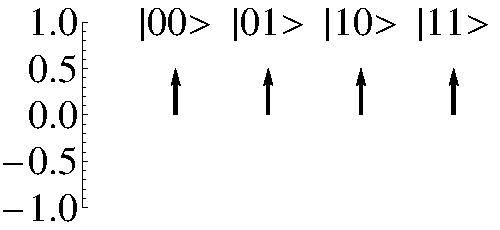
\includegraphics[height=0.2\textheight]{Grovers-equal} 
		} \\
		\; & \(\rightarrow\) & \; \\
		\; & \; & \; \\
	\end{tabular} \\
	\par\medskip
	\item Apply a controlled phase gate \( \rightarrow
		\frac{1}{2}(\ket{00} + \ket{01} + \ket{10} - \ket{11})\) \\
	\begin{tabular}{c c c}
		\multirow{3}{*}{
			\(\left( \begin{array}{cccc}
				1 & 0 & 0 & 0 \\
				0 & 1 & 0 & 0 \\
				0 & 0 & 1 & 0 \\
				0 & 0 & 0 & -1 \\
			\end{array}\right)\)
		} & \; & \multirow{3}{*}{
			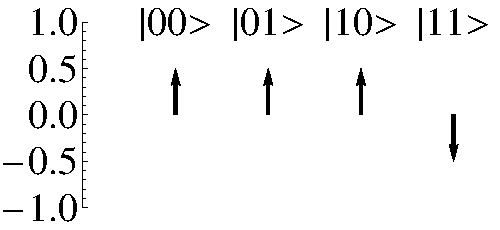
\includegraphics[height=0.2\textheight]{Grovers-marked} 
		} \\
		\; & \(\rightarrow\) & \; \\
		\; & \; & \; \\
	\end{tabular} \\
\end{itemize}
\end{frame}

\begin{frame}{Quantum Computing - Grover's Implementation}
\begin{itemize}
	\item Perform inversion about the mean via two rotations and a controlled phase gate \\
	\par\medskip
	\begin{tabular}{c c c}
		\multirow{3}{*}{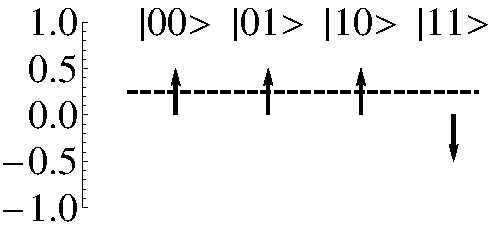
\includegraphics[height=0.2\textheight]{Grovers-inversion1}} & \; & \multirow{3}{*}{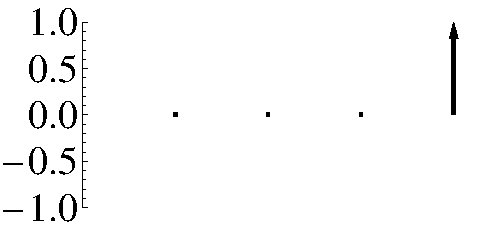
\includegraphics[height=0.2\textheight]{Grovers-inversion2}} \\
		\; & \(\rightarrow\) & \; \\
		\; & \; & \; \\
	\end{tabular}
	\[\mbox{\Tiny \(
	\frac{1}{2} \left( \begin{array}{cccc}
		-1 & 1 & 1 & 1 \\
		1 & -1 & 1 & 1 \\
		1 & 1 & -1 & 1 \\
		1 & 1 & 1 & -1 \\
	\end{array}\right) =
	\frac{1}{\sqrt{2}}\left( \begin{array}{cc}
		1 & 1 \\
		1 & -1 \\
	\end{array}\right)^{\bigotimes 2}
	\left( \begin{array}{cccc}
		1 & 0 & 0 & 0 \\
		0 & -1 & 0 & 0 \\
		0 & 0 & -1 & 0 \\
		0 & 0 & 0 & -1 \\
	\end{array}\right)
	\frac{1}{\sqrt{2}}\left( \begin{array}{cc}
		1 & 1 \\
		1 & -1 \\
	\end{array}\right)^{\bigotimes 2}
	\)}\]
	\item Iterate the previous two steps
\end{itemize}
\end{frame}

\begin{frame}{Quantum Computing - Shor's Algorithm}
Factor integers in \(\mathcal{O}(\log{N})\) time
\begin{itemize}
	\item Can trivially break RSA, a widely used public key encryption algorithm
	\item Classical algorithms significantly faster than \(\approx \mathcal{O}(\sqrt{N})\) are not known
	\item Largest product of two primes ever factored was 768-bits long, took 2000 years of single-core computing
\end{itemize}
\end{frame}

\subsection{MUSIQC}
\begin{frame}{Quantum Computing - MUSIQC}
Modular Universal Scalable Ion-Trap Quantum Computer
\begin{itemize}
	\item Final deliverable planned to have 80 qubits
	\item Plan to have largest possible ion chains in each trap %
		and scale further by linking ions via radiated photons
\end{itemize}
\centerline{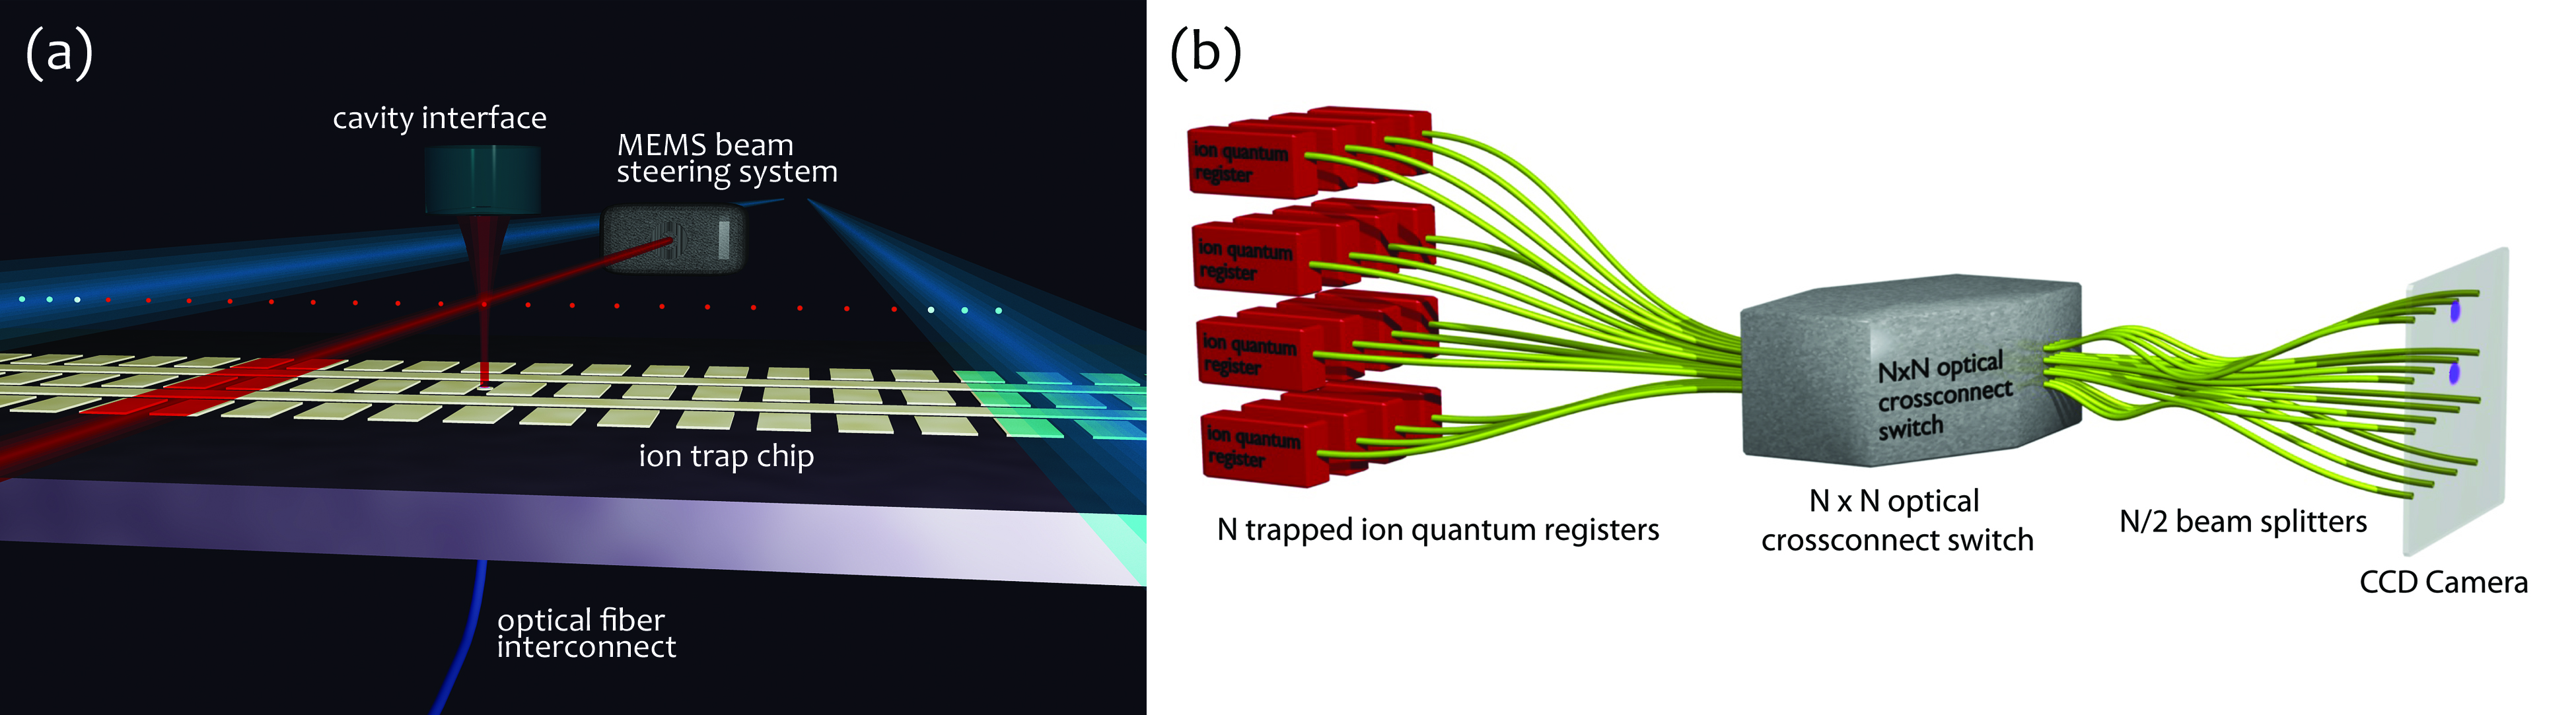
\includegraphics[height=0.45\textheight]{MUSIQC-plan}}
\let\thefootnote\relax\footnote[frame]{C. Monroe, et al, 2012, arXiv:1208.0391}
\end{frame}

\begin{frame}{Quantum Computing - Ions}
\begin{itemize}
	\item Advantages
	\begin{itemize}
		\item Easily trapped and coherently manipulated with easily %
			accessible visible and near-visible transitions
		\item Strong Coulomb coupling allows fast multi-qubit operations
		\item Good environmental isolation allows for long qubit %
			lifetime
		\item Most requirements for quantum computation %
			already demonstrated
	\end{itemize}
	\item Disadvantages
	\begin{itemize}
		\item ``Ion traps don't scale" = Working with increasing %
			numbers of ions to accomplish %
			general quantum computational tasks requires %
			more research
	\end{itemize}
\end{itemize}
\end{frame}

\section{Ion Trapping}
\subsection{Paul Trap}
\begin{frame}{Ion Trapping - Paul Trap RF}
\begin{columns}
	\begin{column}{0.4\textwidth}
		\centerline{\includegraphics[width=0.9\textwidth]%
			{PaulTrap-no_needles}}
	\end{column}

	\begin{column}{0.4\textwidth}
		Considering the center axis of this geometry
		\begin{eqnarray*}
		\phi &=& \frac{1}{2} V \cos( \Omega t ) \frac{x^2 -y^2}{R^2} \\
		\frac{d^2 x}{dt^2} &=& q_x \cos( \Omega t ) x \\
		\frac{d^2 y}{dt^2} &=& -q_y \cos( \Omega t ) y
		\end{eqnarray*}
	\end{column}
\end{columns}
\end{frame}

\begin{frame}[label=micromotion]{Ion Trapping - Paul Trap RF}
	\[ \frac{d^2 x}{dt^2} = -q_x \cos( \Omega t ) x
		\; (- c_x) \]
	\begin{center}\begin{tabular*}{0.9\textwidth}{@{\extracolsep{\fill}} cc}
		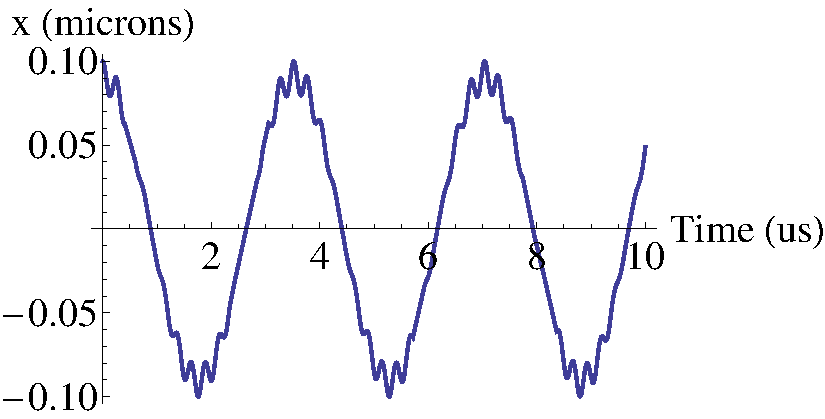
\includegraphics[width=0.45\textwidth]{PaulTrap-ion_motion} &
		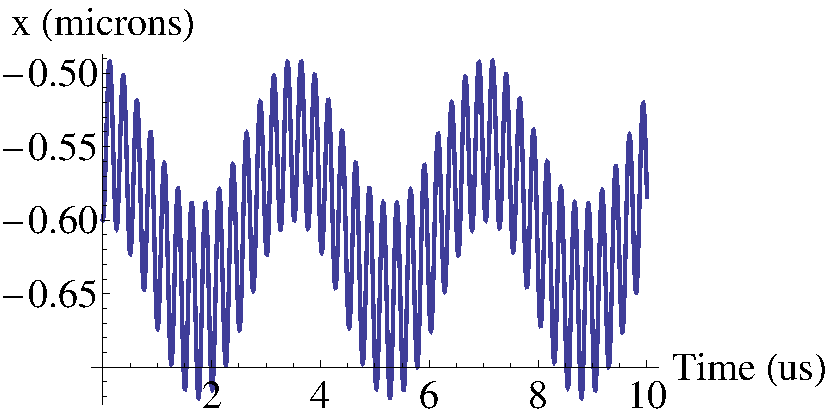
\includegraphics[width=0.45\textwidth]{PaulTrap-micromotion} \\
		Trap centered on rf null &
		Trap offset from null \\
	\end{tabular*}\end{center}
	The large amplitude motion can be shown from the Mathieu
	equation to correspond to a harmonic trap with 
	\( \omega_{x,y} = \frac{q V}{\sqrt{2} \Omega^2 m R^2} \)
	with some stability conditions on the strength of rf and dc
	signals.
\end{frame}

\begin{frame}{Ion Trapping - Paul Trap DC}
\begin{columns}
	\begin{column}{0.4\textwidth}
		\centerline{\includegraphics[width=0.9\textwidth]%
			{PaulTrap}}
	\end{column}
	\begin{column}{0.4\textwidth}
		Confinement along the axial direction is achieved by applying
		DC voltage to needles
		\begin{eqnarray*}
		\phi &=& k U (z^2 - \frac{1}{2} (x^2 + y^2)) \\
		\omega_z &=& \sqrt{\frac{2 k q U}{m}}
		\end{eqnarray*}
		Weaker confinement than RF
	\end{column}
\end{columns}
\end{frame}

\begin{frame}{Ion Trapping - Ion Chains}
	To build a quantum computer we want to trap and interact with a 
	large number of ions.
	\centerline{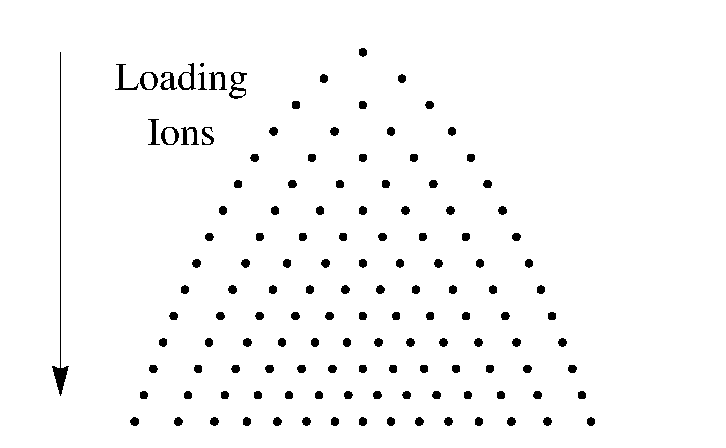
\includegraphics[height=0.25\textheight,width=0.4\textwidth]{Chains-spacing}}
	Continue until \( \frac{\omega_{x,y}}{\omega_z} \approx 0.6 N^{0.86} \)
	\let\thefootnote\relax\footnote[frame]
		{Wineland, 1998, arXiv:quant-ph/9710025v2}
	\begin{center}
		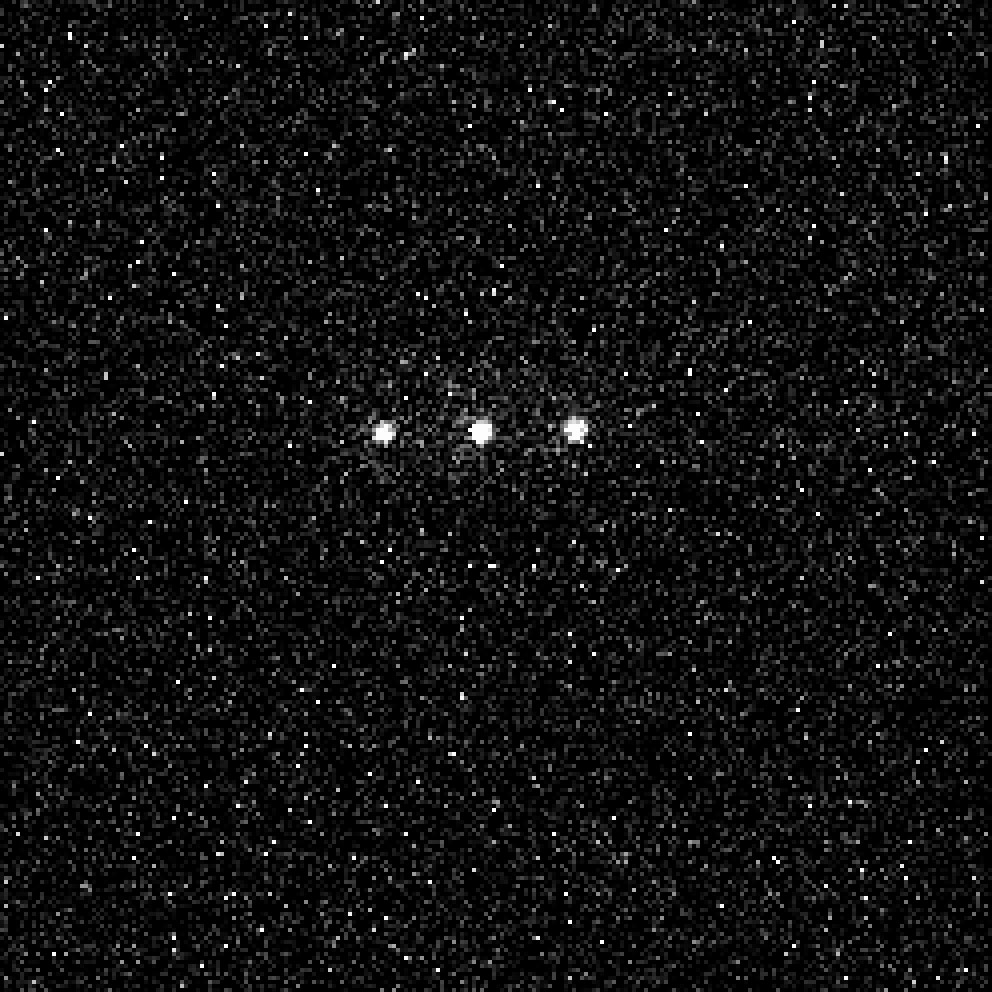
\includegraphics[height=0.3\textheight]{ThreeIons}
		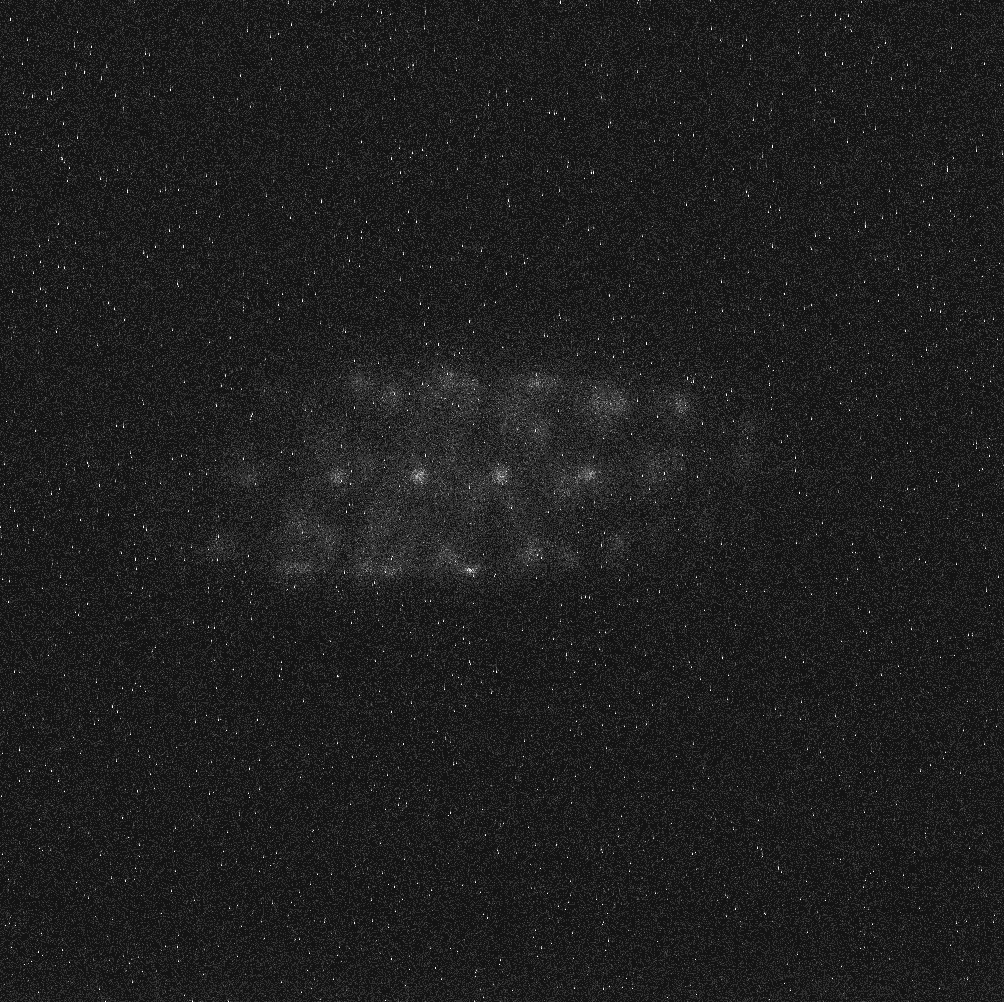
\includegraphics[height=0.3\textheight]{BigChain}
	\end{center}
\end{frame}

\begin{frame}{Ion Trapping - Anharmonic Ion Chains}
To avoid zig-zag transition want to control axial potential
\begin{columns}
	\begin{column}{0.4\textwidth}
		\centerline{
			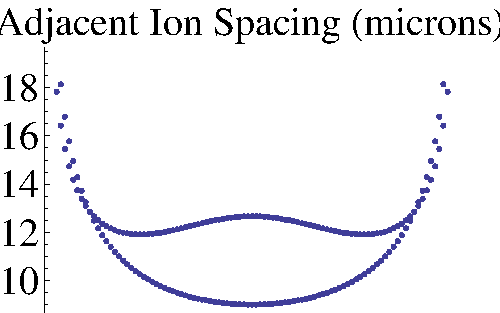
\includegraphics[width=0.9\textwidth]{Chains-quartic_spacing3}}
		{\scriptsize Spacing between adjacent ions in harmonic trap and optimized quartic trap}
	\end{column}
	\begin{column}{0.6\textwidth}
\begin{eqnarray*}
	V_z(z) &=& a z^2 + b z^4 \\
	U_z &=& \sum_{i=1}^N V_z(z_i) + \sum_{j<i} \frac{e^2}{4 \pi \epsilon_0 \abs{z_i - z_j}} \\
\end{eqnarray*}
	More equally spaced ion chains limit the higher frequency axial modes
	and allow stable trapping with easily achievable rf power
	\let\thefootnote\relax\footnote[frame]
		{G.-D. Lin et al 2009 EPL 86 60004}
	\end{column}
\end{columns}
\end{frame}

\subsection{Surface Trap}
\begin{frame}{Ion Trapping - Surface Trap}
\begin{columns}
	\begin{column}{0.4\textwidth}
		\centerline{\includegraphics[width=0.9\textwidth]%
			{GenIIIPackage-GTRI_GenIII_Overview}}
	\end{column}
	\begin{column}{0.6\textwidth}
		\begin{itemize}
			\item 96 independent electrodes in standardized CPGA socket
			\item Reproducability will help improve scalablity
			\item Manufactured for MUSIQC by Sandia and GTRI
		\end{itemize}
	\end{column}
\end{columns}
\end{frame}

\begin{frame}{Ion Trapping - Surface Trap Geometries}
\begin{center}
	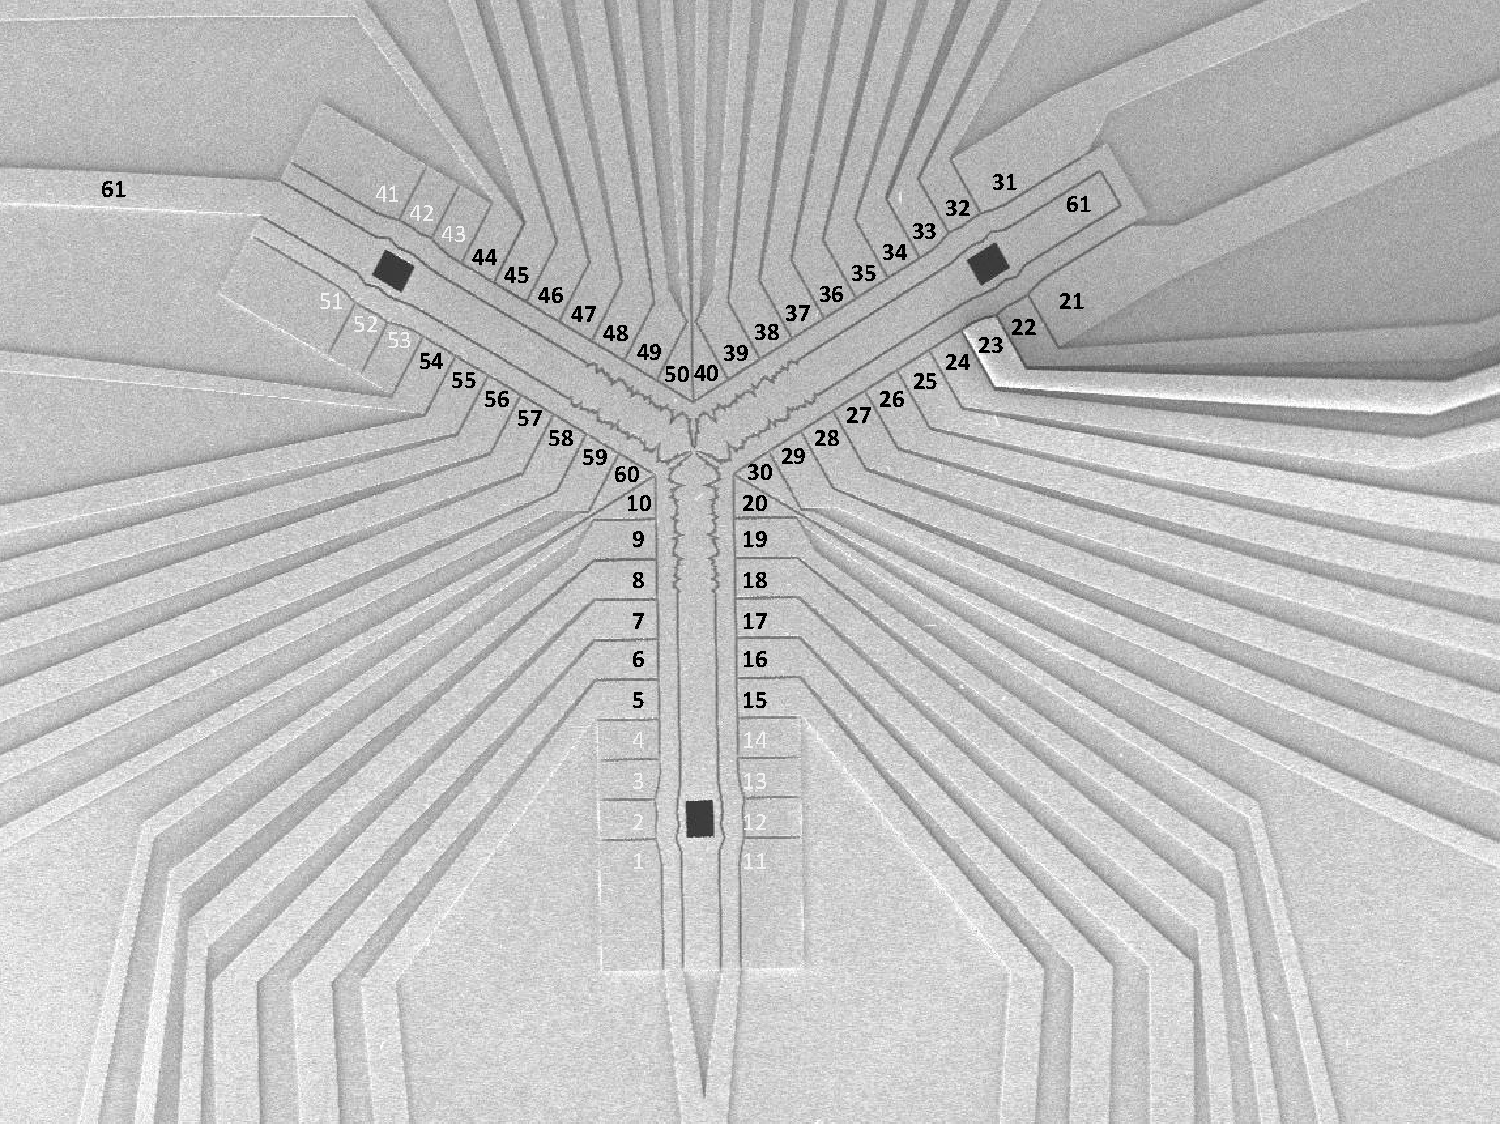
\includegraphics[height=0.7\textheight]{electrode_assignment_Yu-1}
\end{center}
\end{frame}

\begin{frame}{Ion Trapping - Surface Trap Fabrication}
\centerline{\includegraphics[width=1.0\textwidth]%
	{ChipTrapFab-GTRI_GenIII_Overview}}
\end{frame}

\section{Experimental Setup}
\subsection{Apparatus}
\begin{frame}{Experimental Setup - Introduction}
Obligatory experimentalist inclusion
\begin{center}
	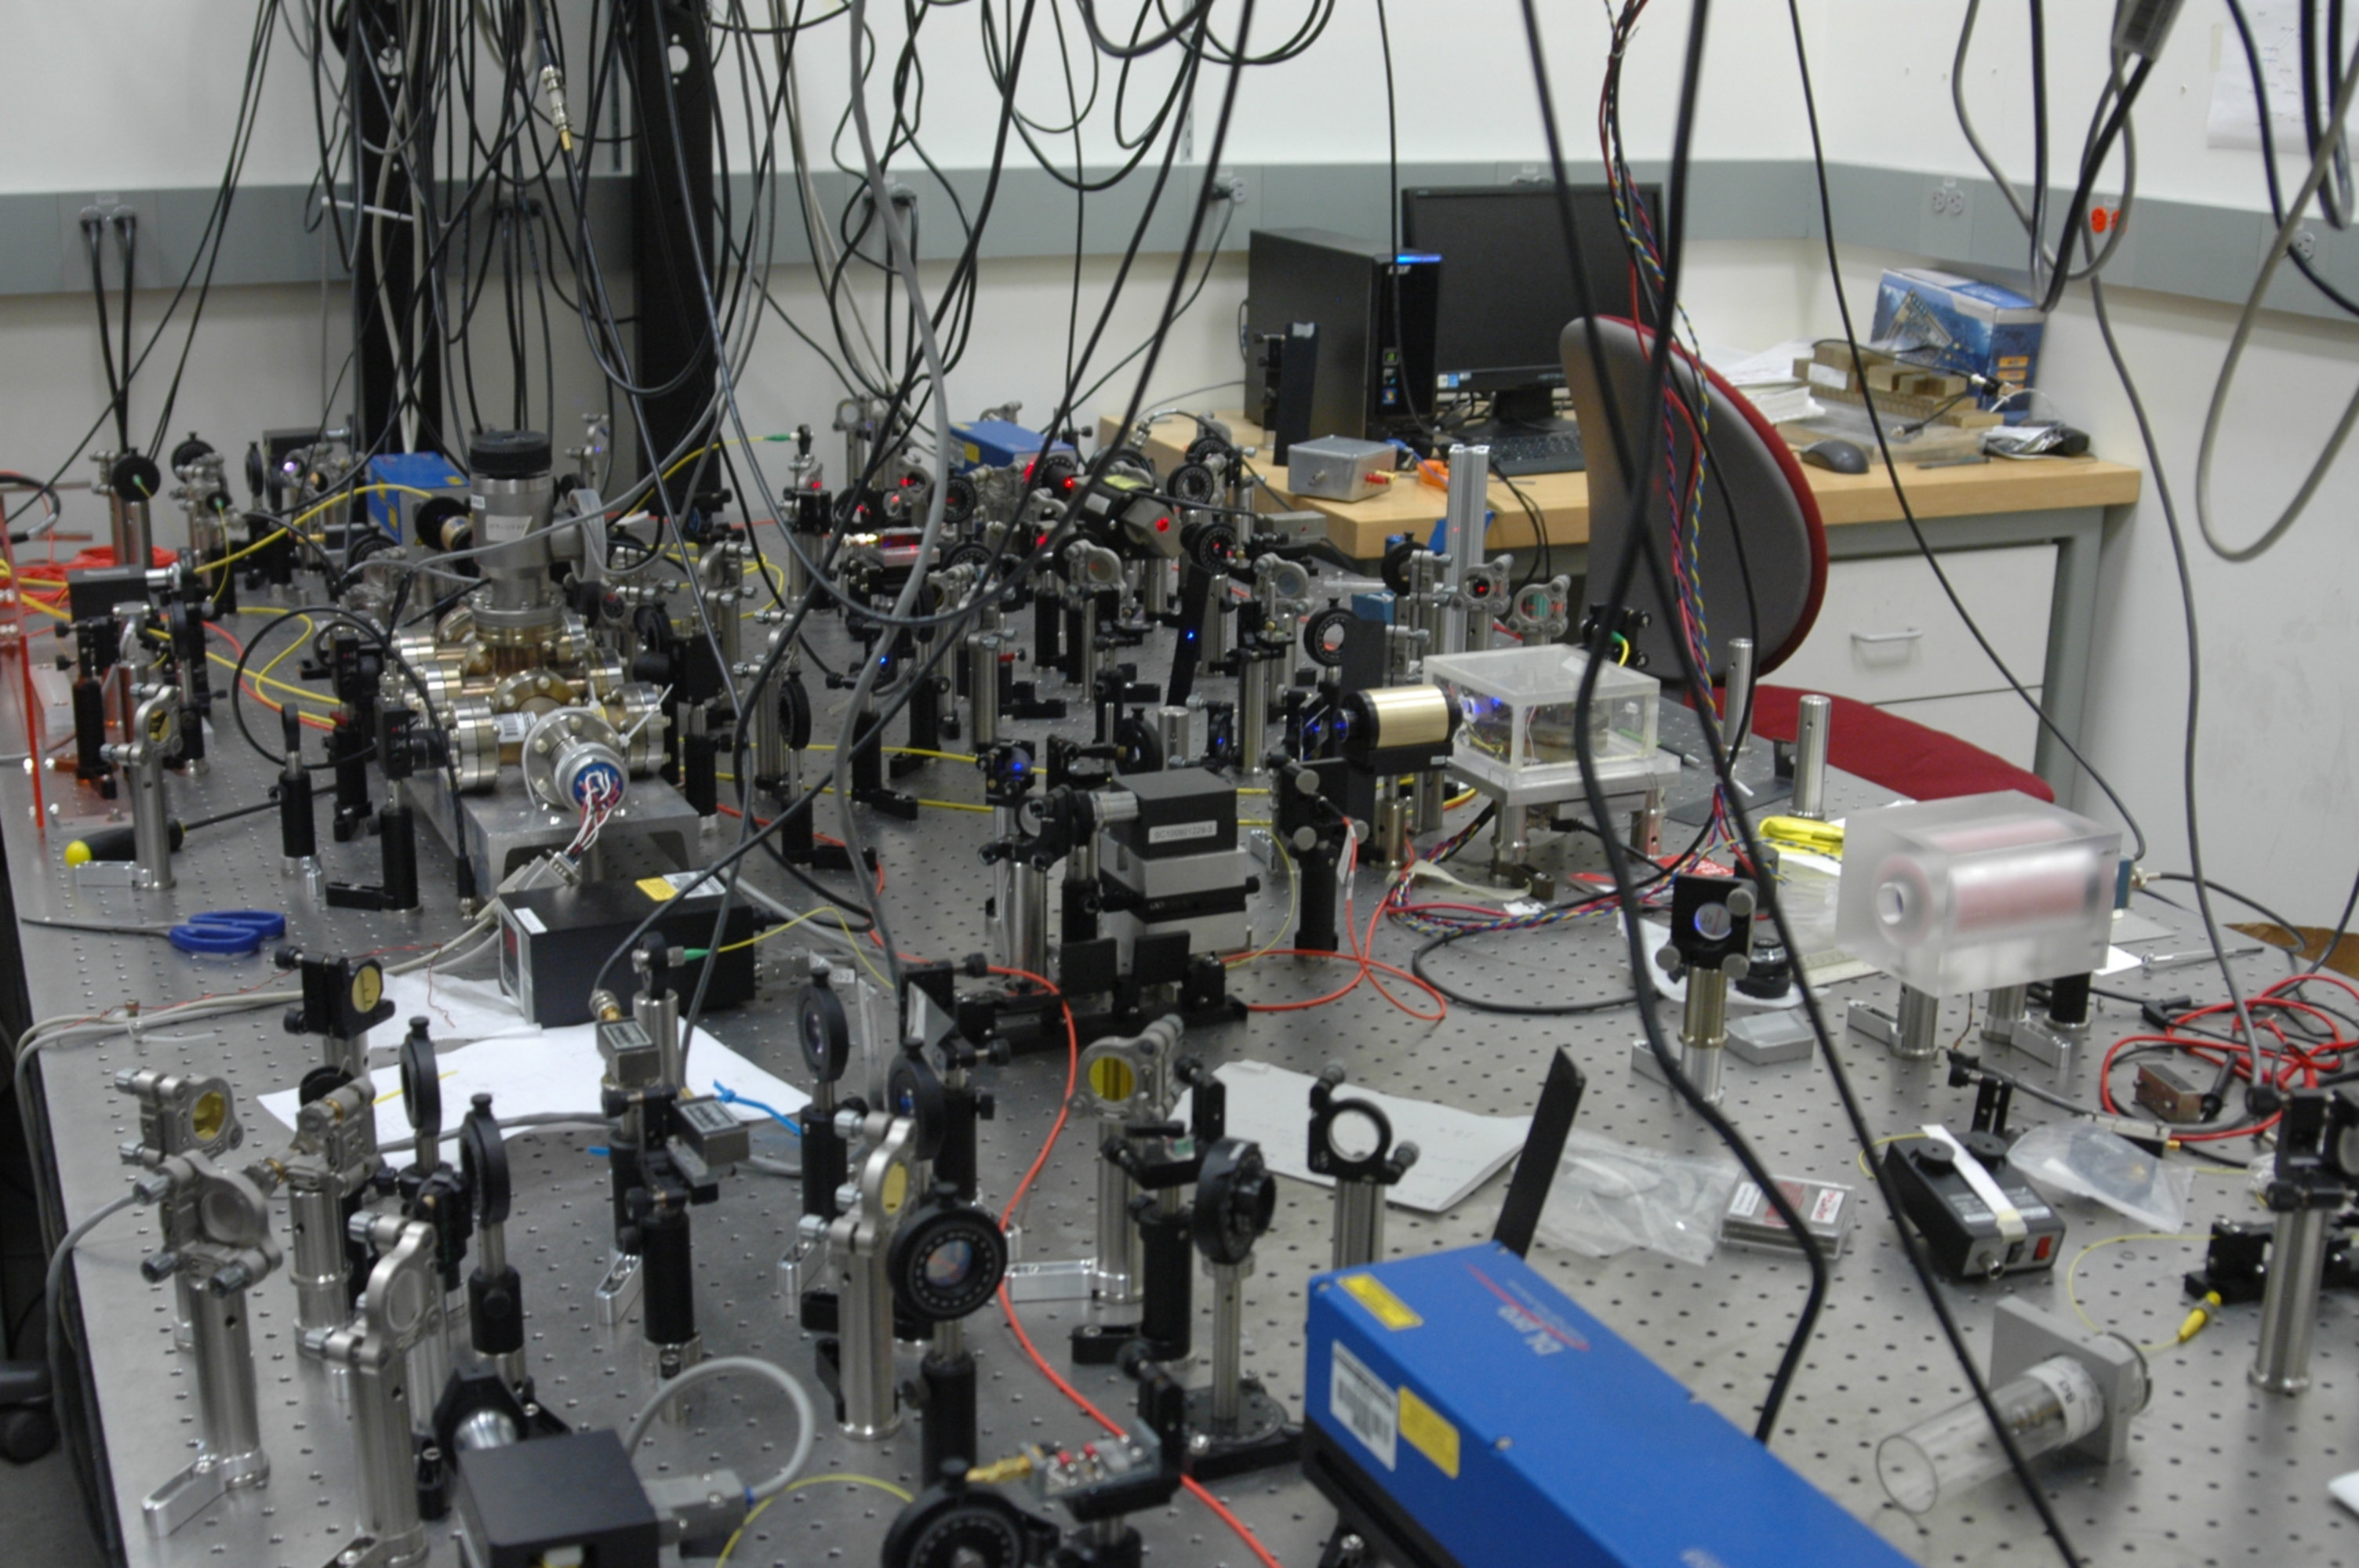
\includegraphics[width=0.5\textwidth]{camera/laser_table}
	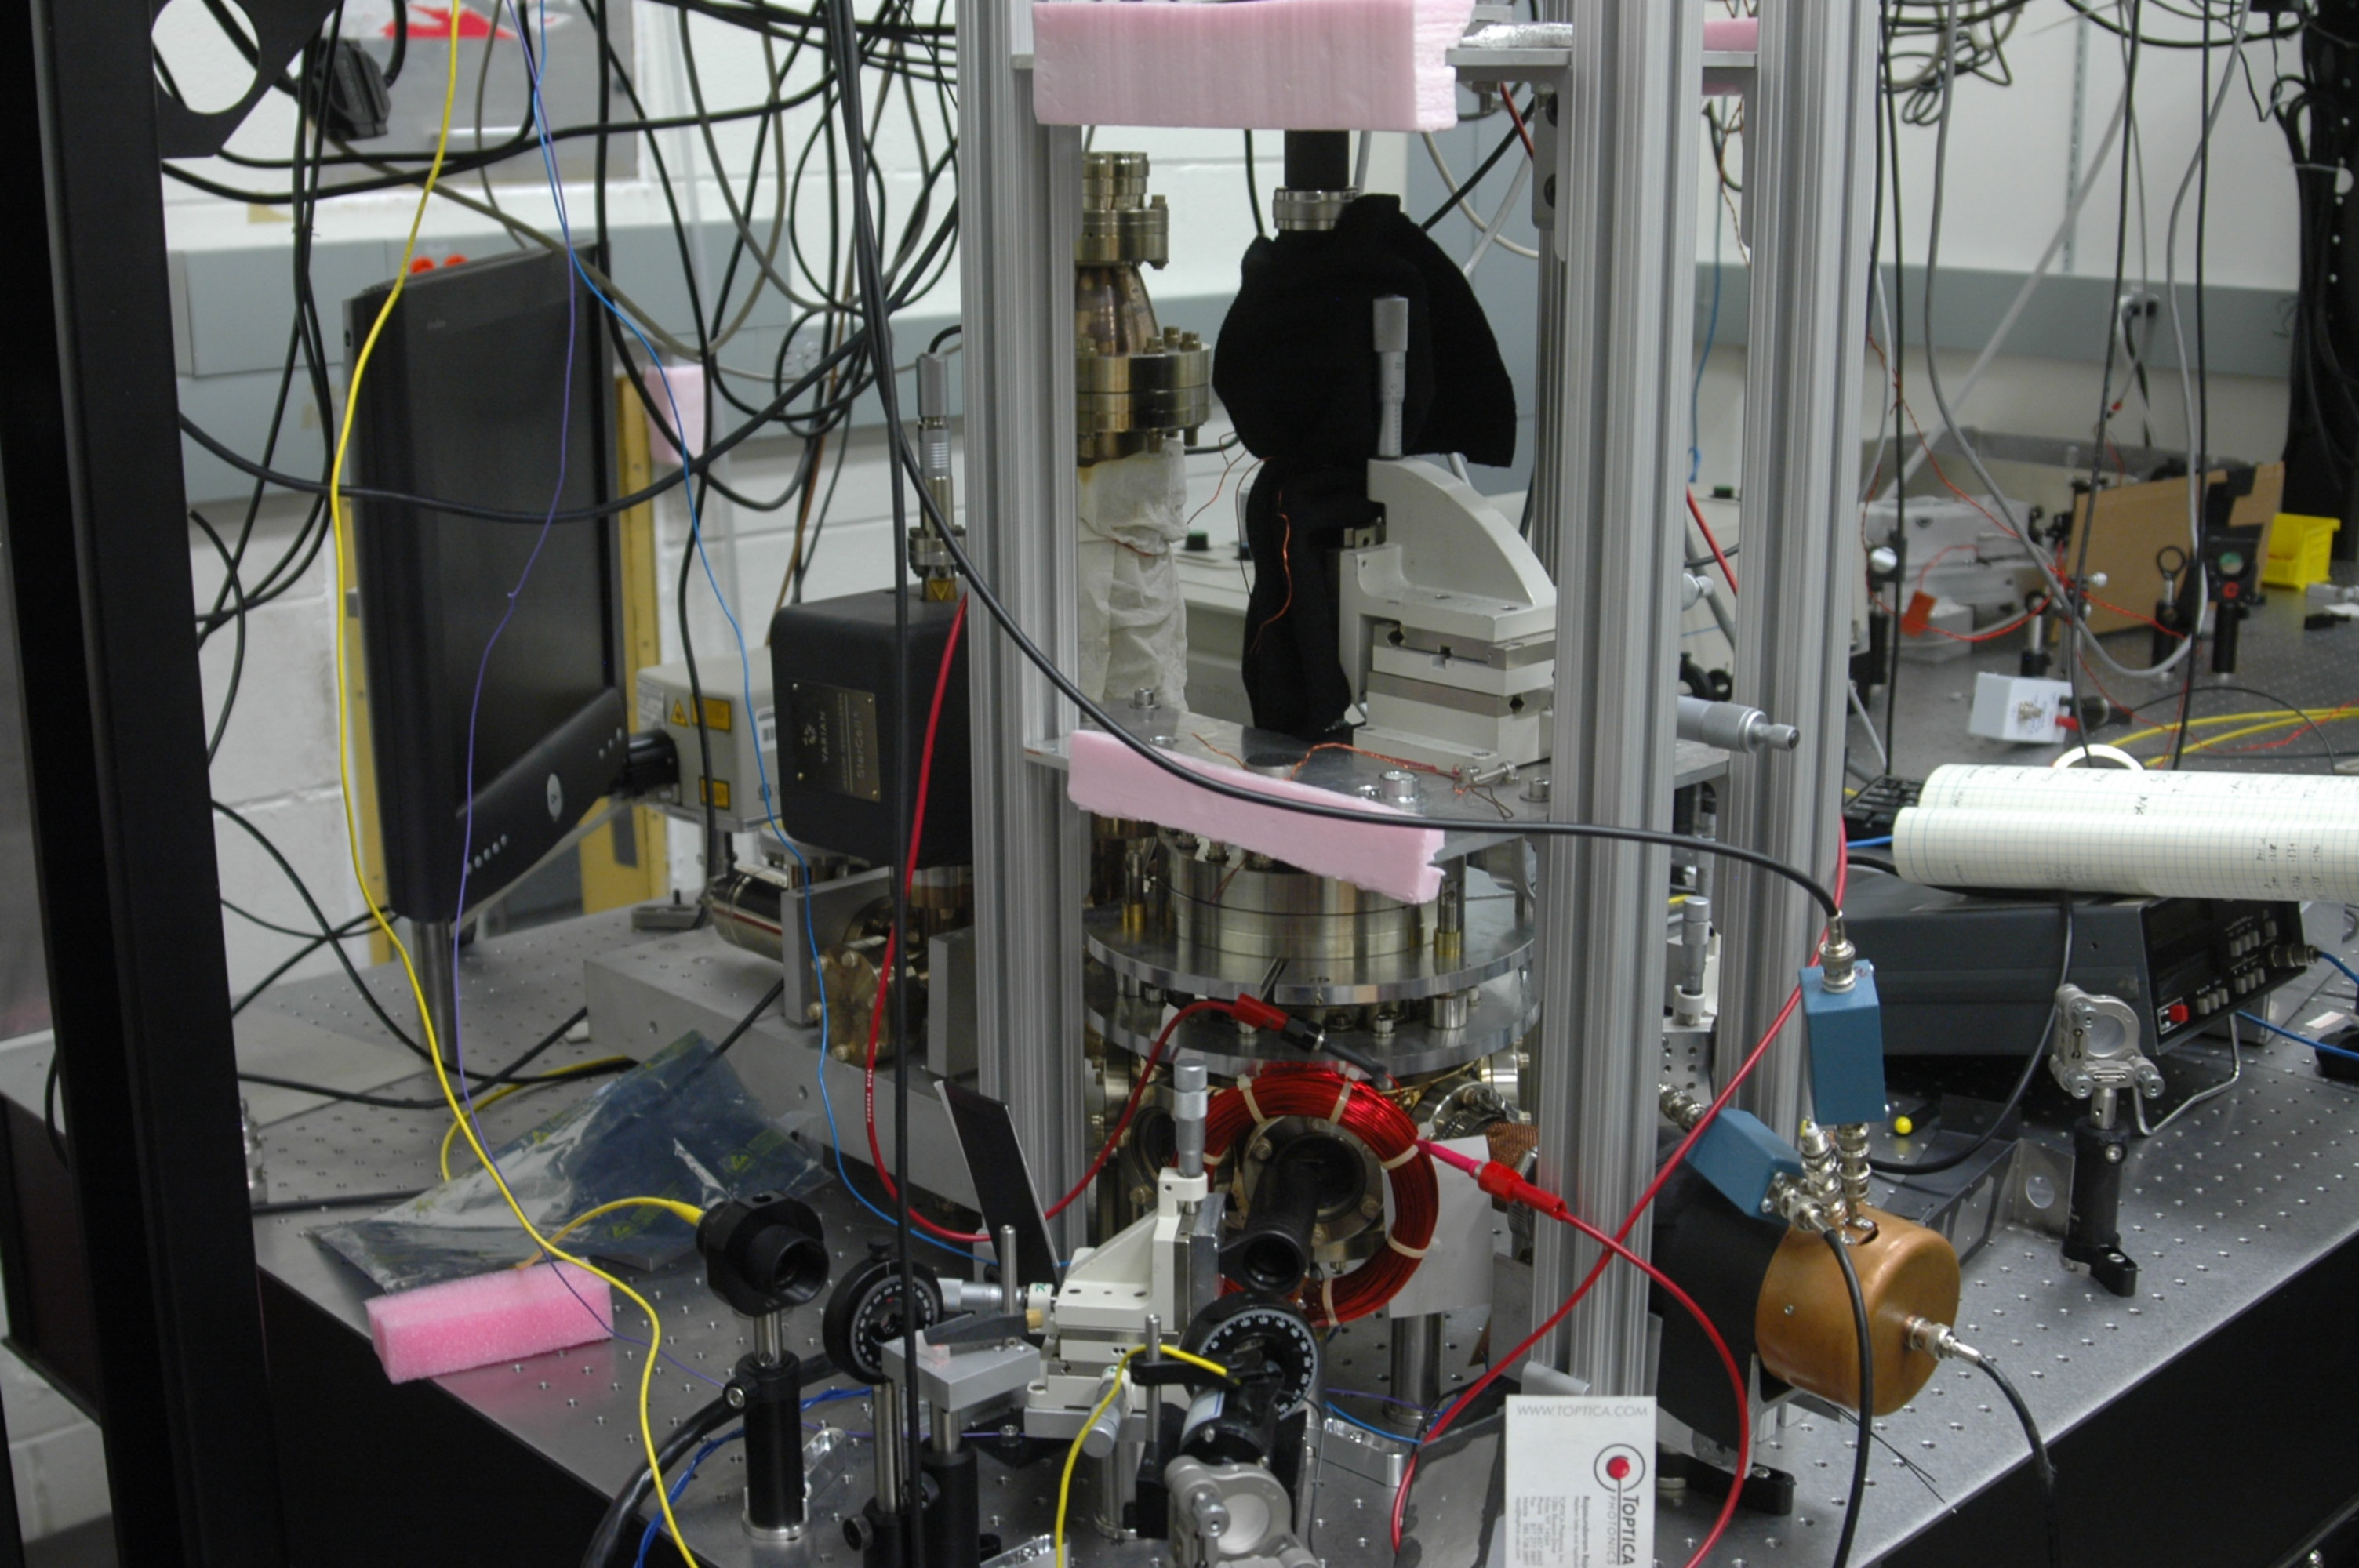
\includegraphics[width=0.5\textwidth]{camera/macro_trap}
\end{center}
\end{frame}

\begin{frame}{Experimental Setup - Surface Trap Chamber}
\begin{columns}
	\begin{column}{0.4\textwidth}
		\centerline{\includegraphics[width=1.0\textwidth]%
			{chiptrap-chamber}}
	\end{column}
	\begin{column}{0.6\textwidth}
		\begin{itemize}
			\item ZIF socket allows for easy chip swapping
			\item In-vacuum capacitors filter rf from DC electrodes
			\item DC connections routed through DSUB-25 connectors
		\end{itemize}
	\end{column}
\end{columns}
\end{frame}

\begin{frame}{Experimental Setup - DC Control}
\begin{itemize}
	\item 96 DC electrodes need to be updated precisely and rapidly
\end{itemize}
\begin{columns}
	\begin{column}{0.4\textwidth}
		\centerline{\includegraphics[width=0.9\textwidth]%
			{camera/DAC_board}}
	\end{column}
	\begin{column}{0.6\textwidth}
		\begin{itemize}
			\item Computer loads DC potentials into FPGA SRAM
				over UDP interface
			\item FPGA can be triggered to upload static or
				dynamic clocked potentials over serial
				interface to 32-channel DACs
			\item Update rate up to 2 MHz/channel or
				200 kHz/potential step
		\end{itemize}
	\end{column}
\end{columns}
\end{frame}

\begin{frame}{Experimental Setup - Surface Trap Potentials}
96 DC control electrodes allows us to work with long chains
\begin{itemize}
	\item Establish loading zones to continuously load ions for later
		use
	\item Loaded ions can be held in a different zone until needed
	\item Chains of different ion species or isotopes can be reordered
	\item Potentials that allow long linear chains while avoiding the
		zig-zag transition
\end{itemize}
\end{frame}

\subsection{Engineering Challenges}
\begin{frame}{Experimental Setup - Engineering Challenges}
Trapping in chip traps has involved some engineering challenges
\begin{itemize}
	\item 96 DC electrodes need to be updated precisely and rapidly
	\item In-vacuum PCB traces developed microfractures from chip insertion force
	\item UV beams near the chip surface cause charging
	\item Small loading holes can be blocked by large Ba deposits
\end{itemize}
\end{frame}

\begin{frame}{Experimental Setup - UV Charging}
\begin{itemize}
	\item UV beams near the chip surface cause charging
\end{itemize}
\begin{center}
	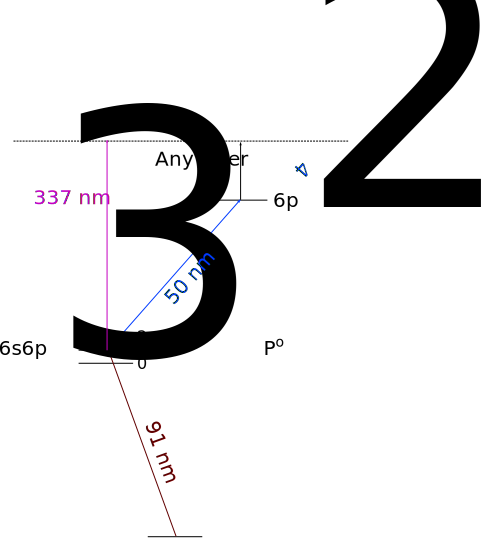
\includegraphics[height=0.5\textheight]{energylevels-neutral}
	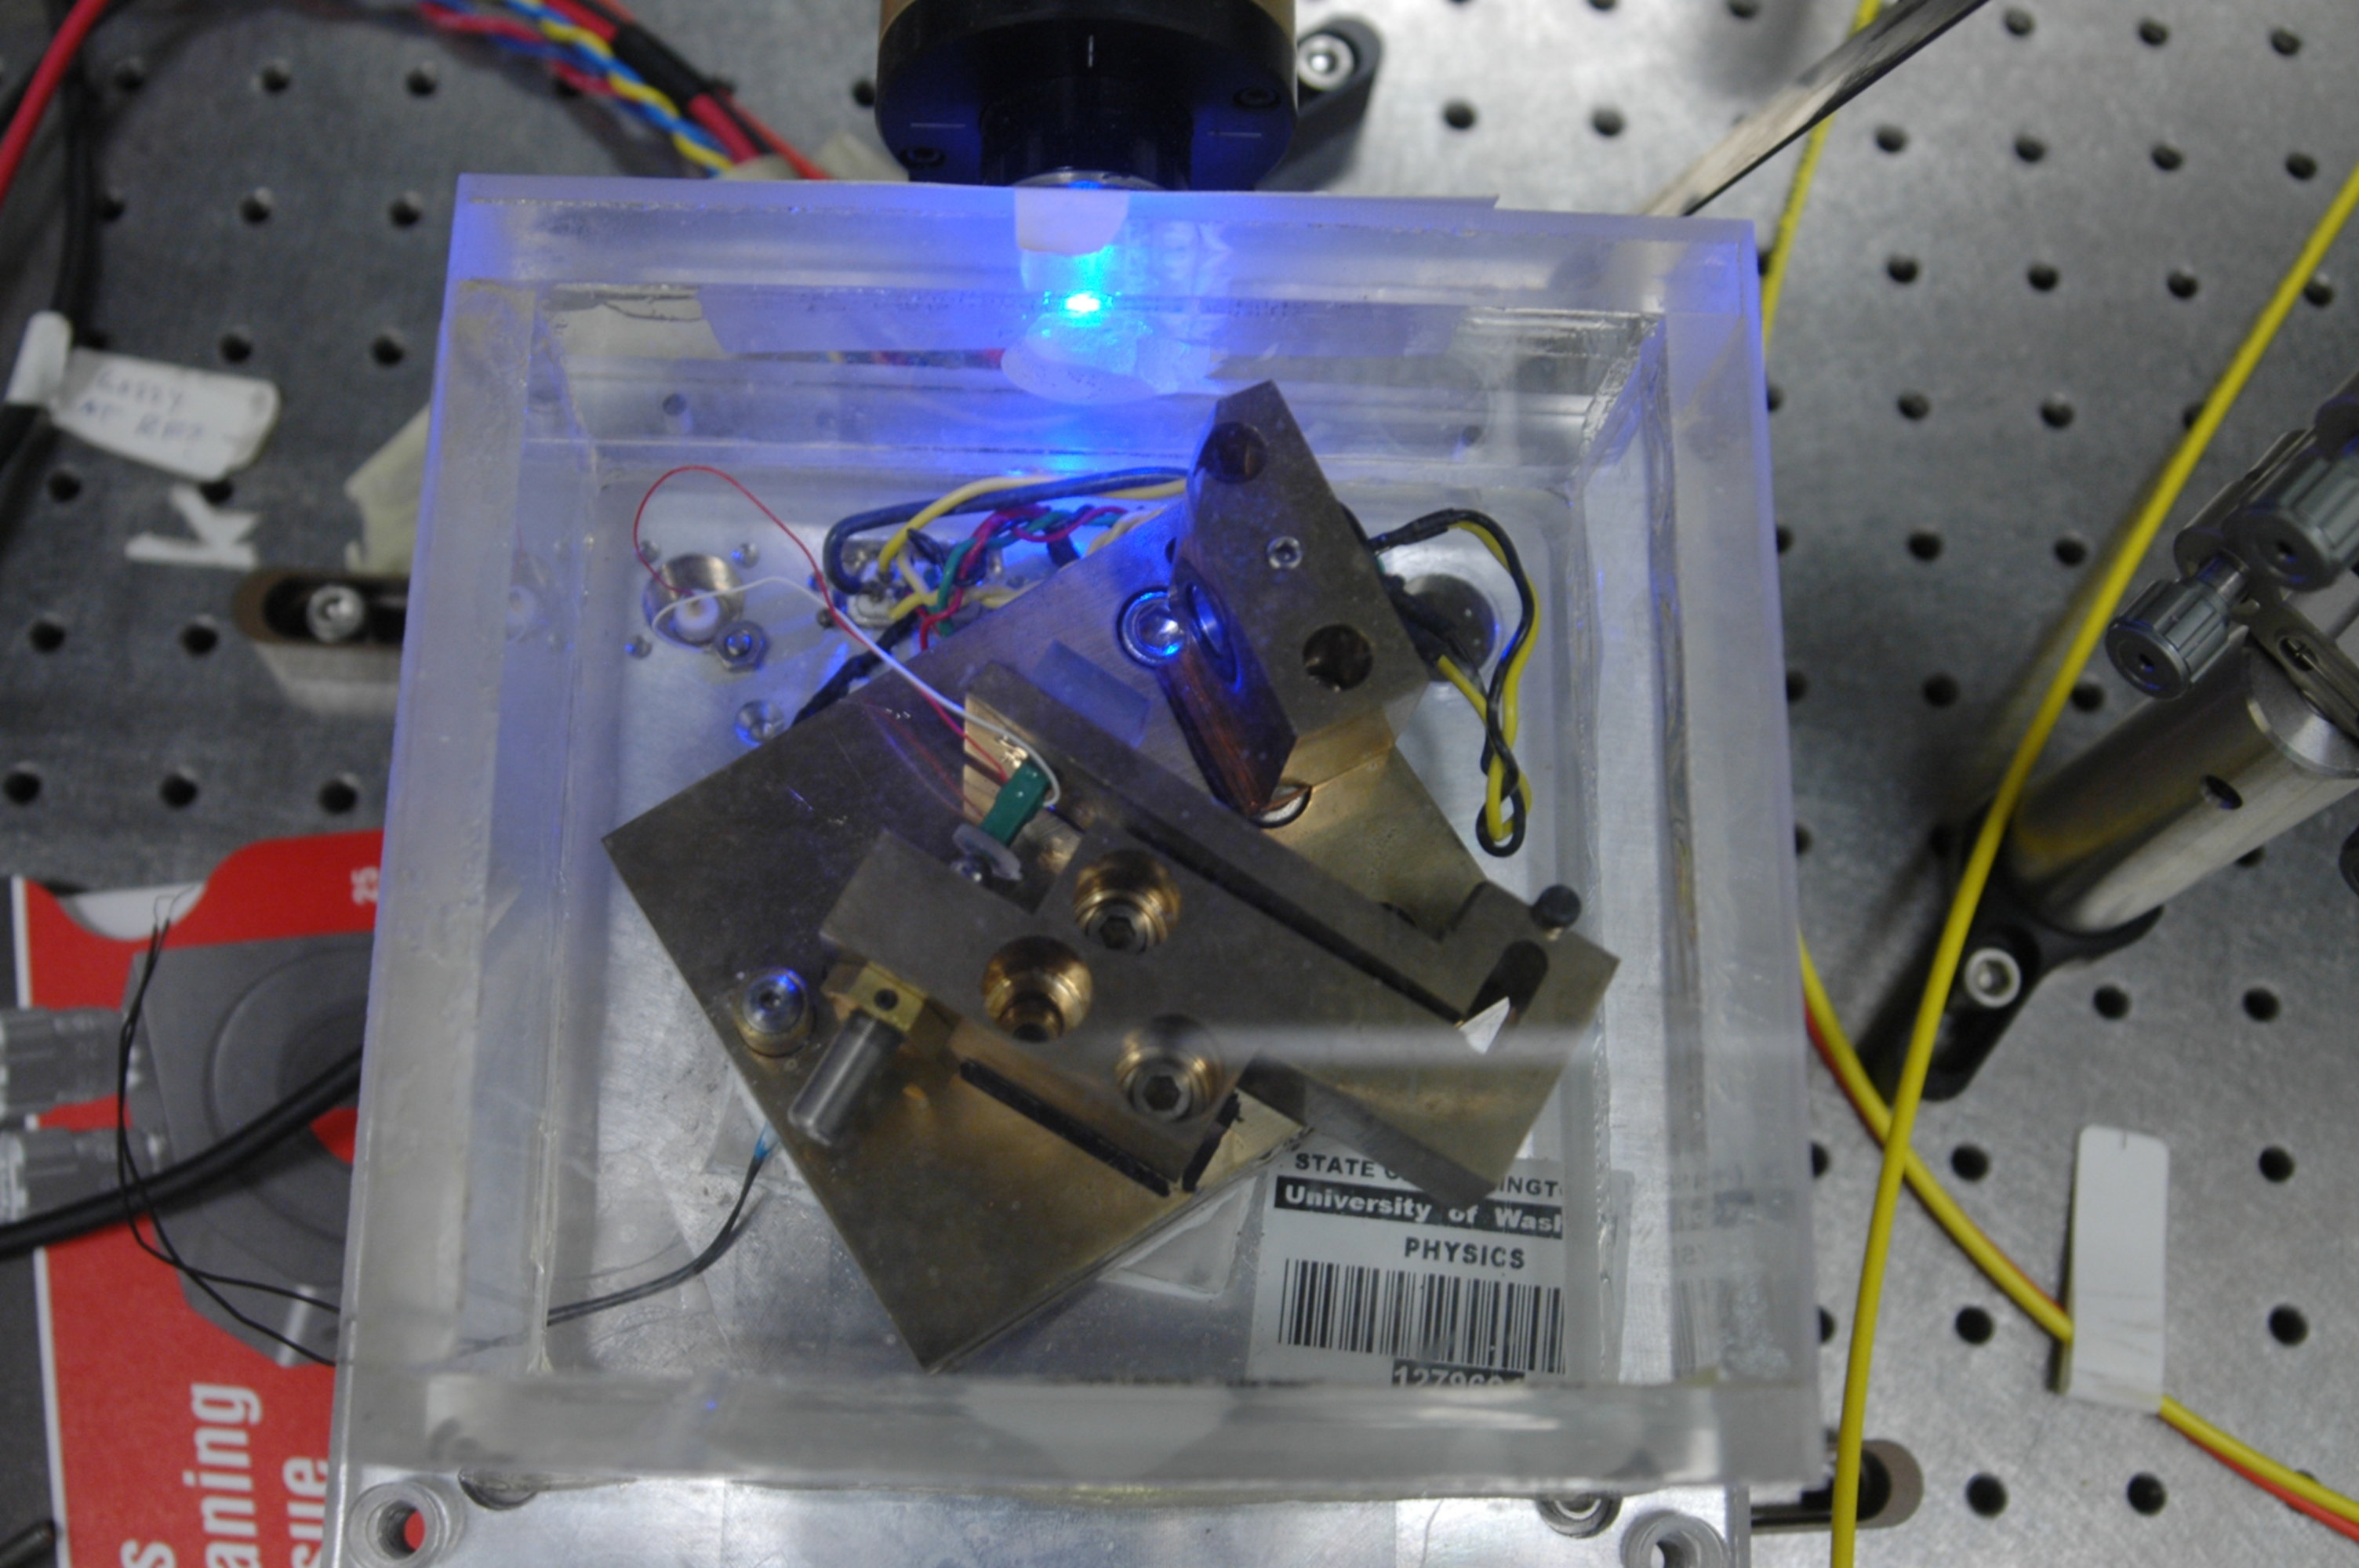
\includegraphics[height=0.5\textheight]{camera/450_laser}
\end{center}
\end{frame}

\begin{frame}{Experimental Setup - Barium Deposition}
\begin{itemize}
	\item Small loading holes can be blocked by large Ba deposits
\end{itemize}
\begin{columns}
	\begin{column}{0.4\textwidth}
	\begin{center}
		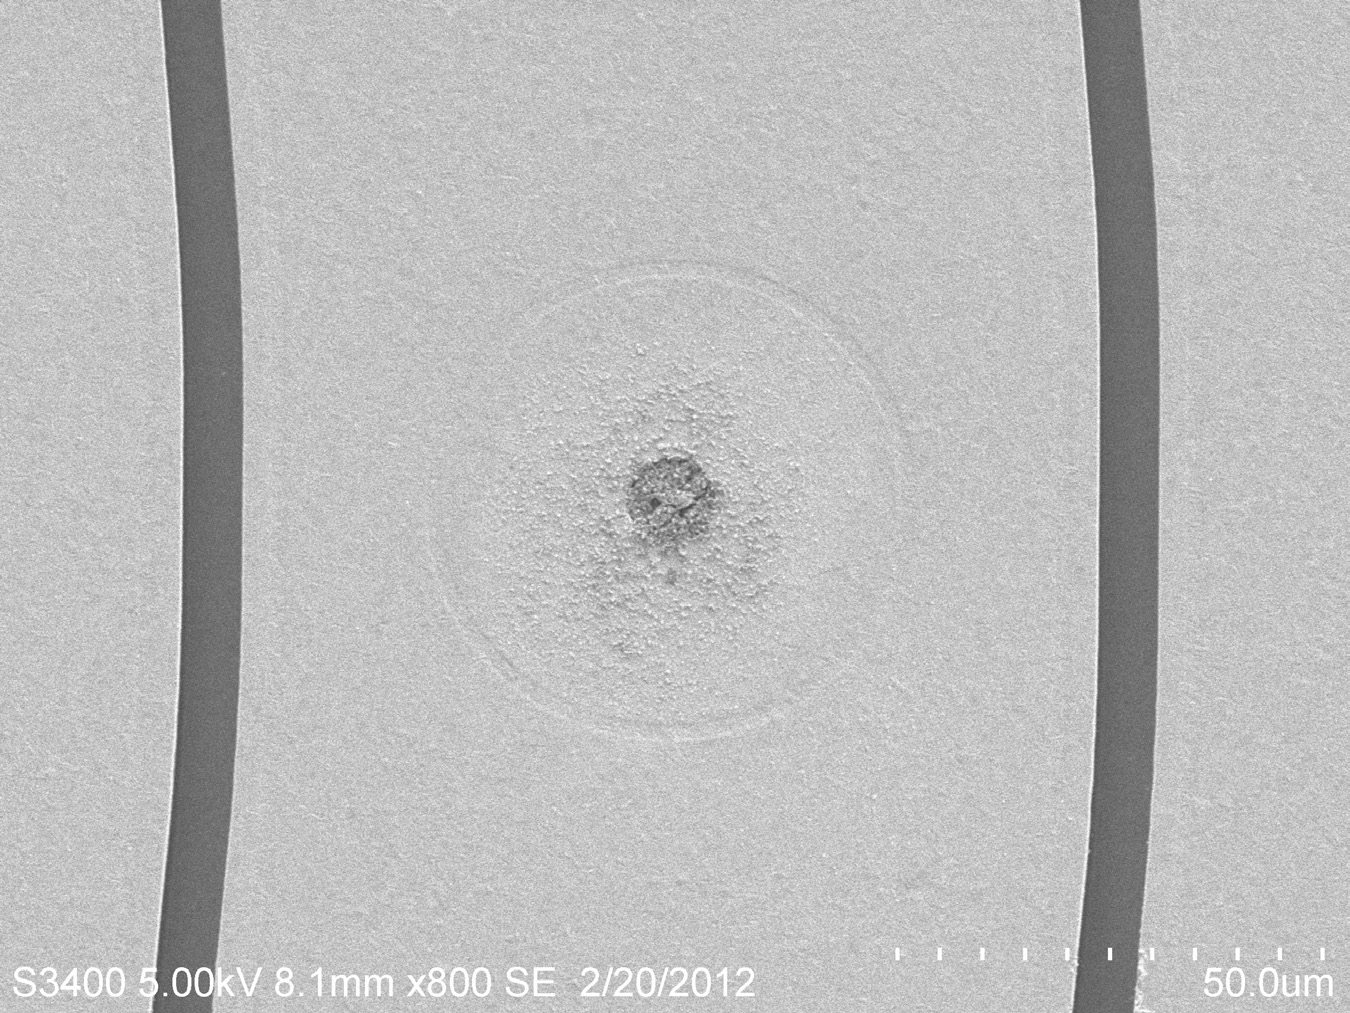
\includegraphics[width=0.8\textwidth]{RingTrap-blocked}
		\vfill
		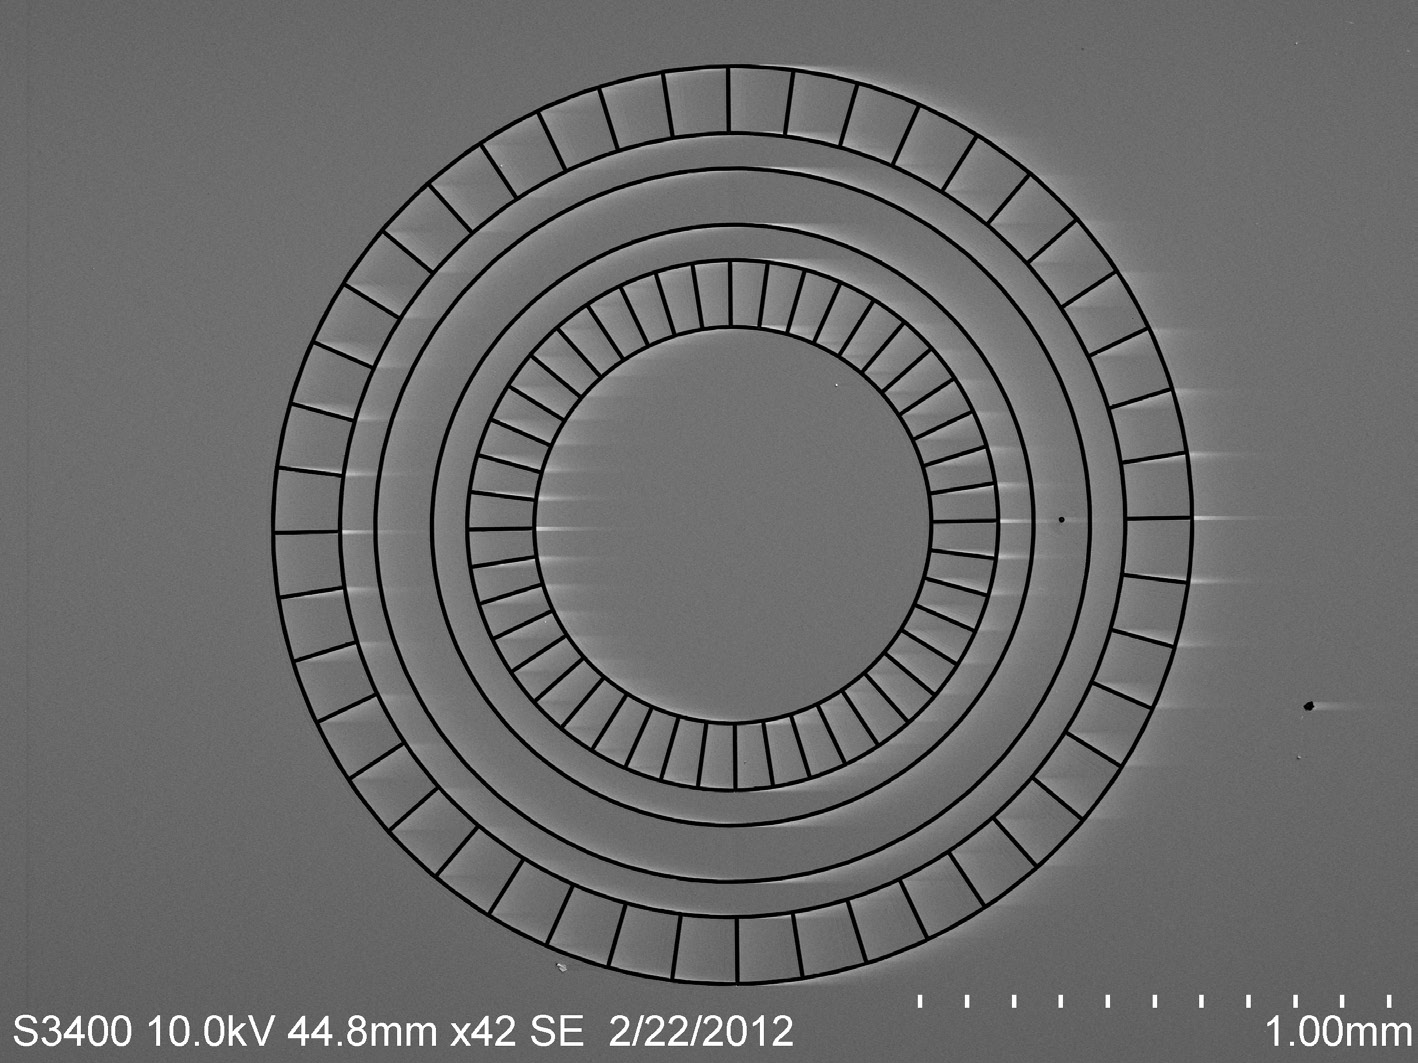
\includegraphics[width=0.8\textwidth]{RingTrapSEM}
	\end{center}
	\end{column}
	\begin{column}{0.6\textwidth}
		\begin{itemize}
			\item Ba oxidation in oven requires priming oven at %
				very high temperatures
			\item Commercial Ba ovens avoid this problem
			\item Bimetallic oven shield can be actuated in vacuum %
				to shield trap from oven
		\end{itemize}
	\end{column}
\end{columns}
\end{frame}

\section{Experimental Results}
\begin{frame}{Experimental Results - Initial Trapping}
\begin{center}
	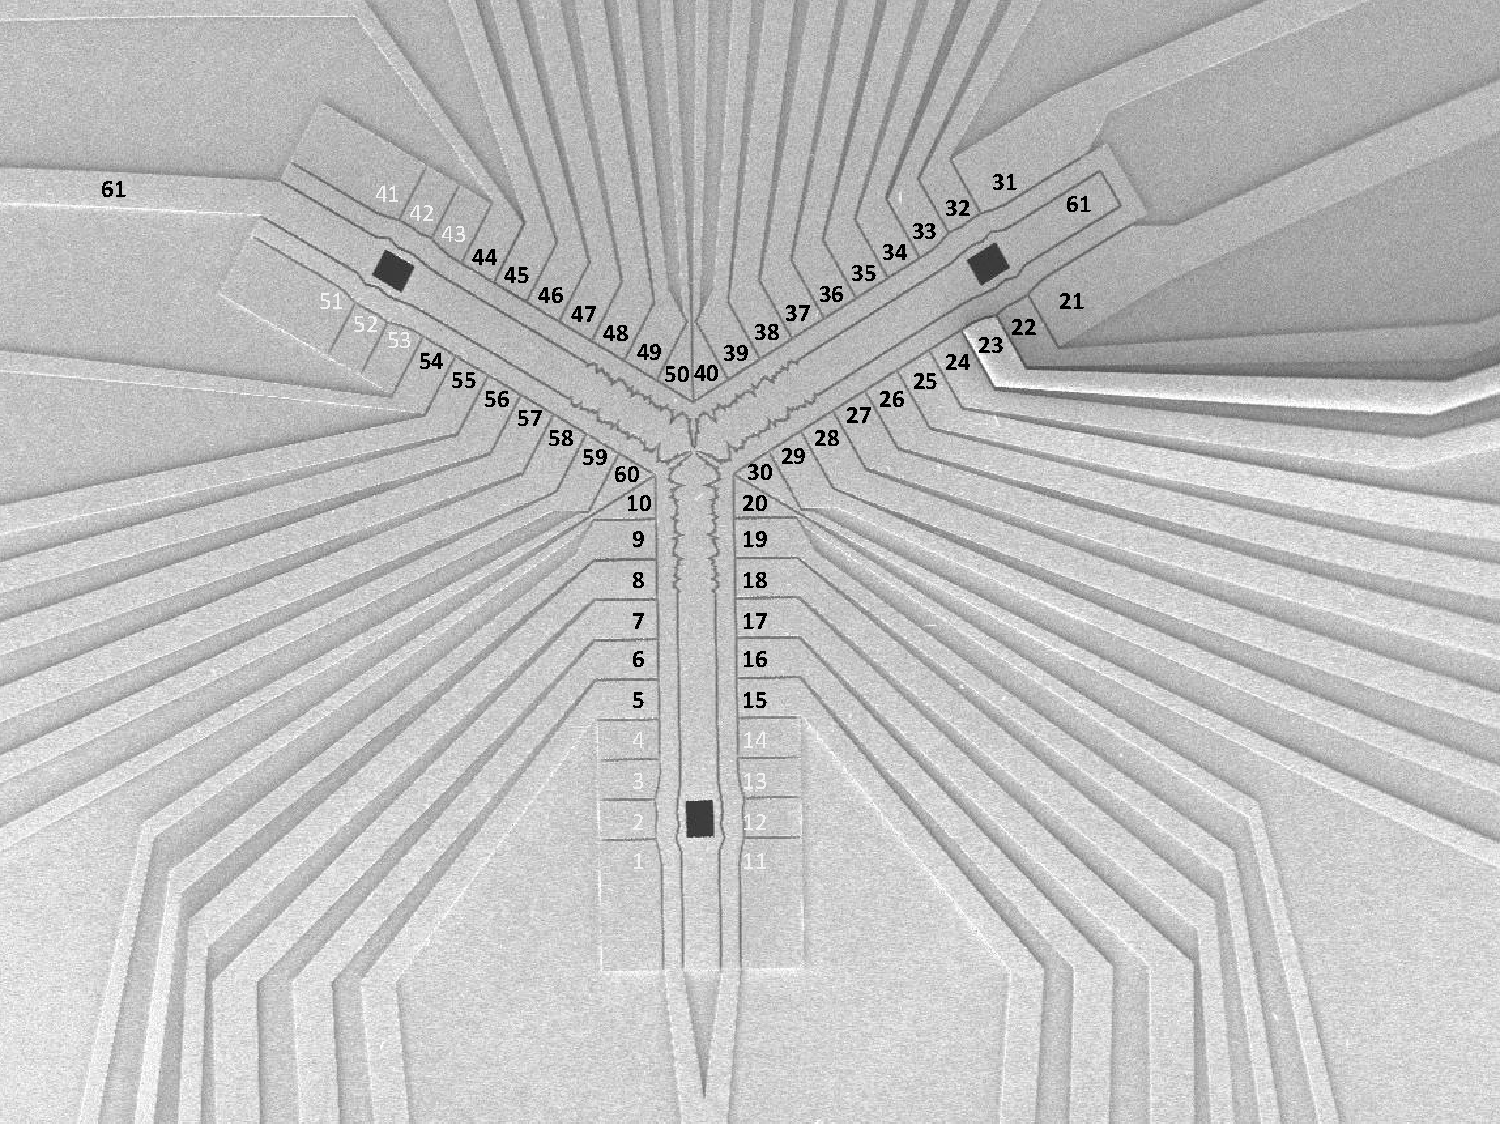
\includegraphics[height=0.5\textheight]{electrode_assignment_Yu-1}
	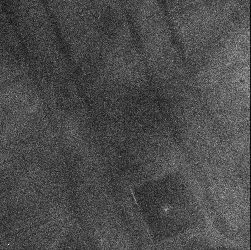
\includegraphics[height=0.5\textheight]{NoSecondStage}
\end{center}
\end{frame}

\subsection{Results}
\begin{frame}{Experimental Results - Shuttling}
\centerline{
	\movie[externalviewer]
		{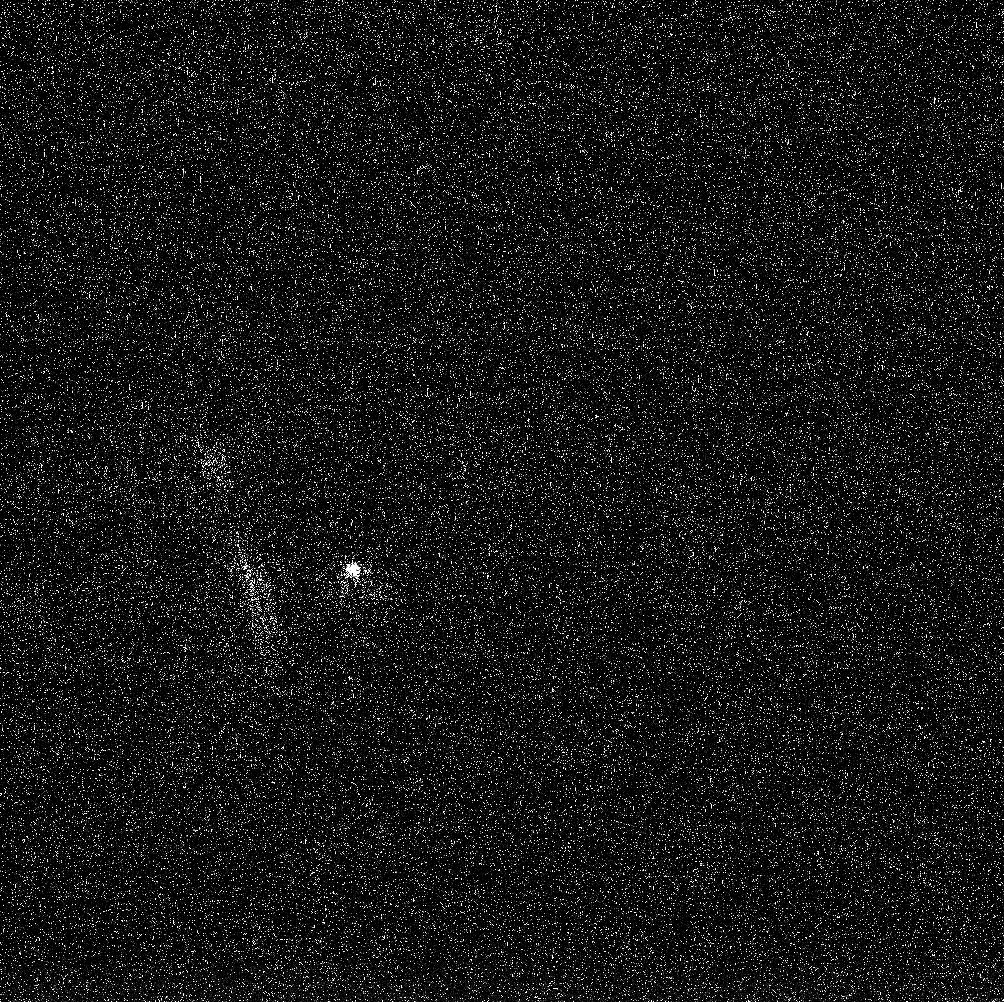
\includegraphics[height=0.6\textwidth]{loading_hole_position}}
	{ion_shuttle.mpg}}
\end{frame}

\begin{frame}{Experimental Results - Lifetime}
High heating rates in surface traps has made ion dark lifetime problematic
in the past, but our measured lifetimes of \(\approx\)30 seconds should
be sufficient.
\par\medskip
\centerline{\begin{tabular*}{0.9\textwidth}{cc}
	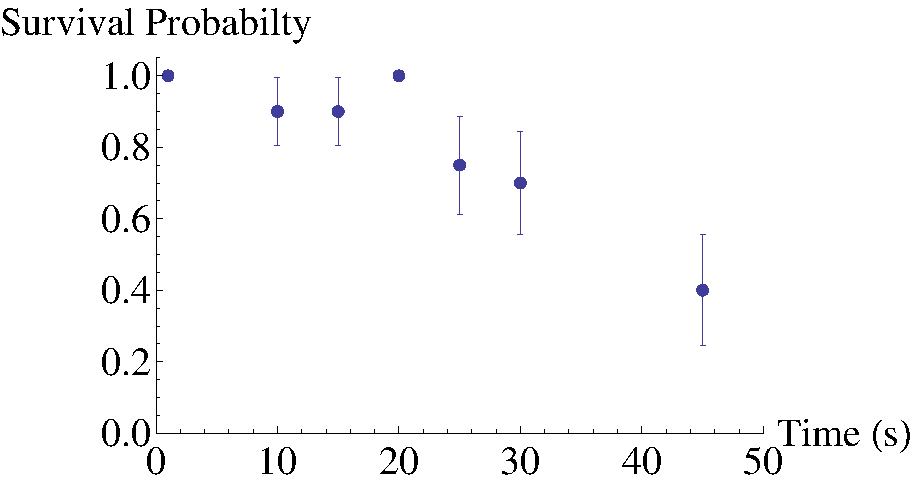
\includegraphics[width=0.45\textwidth]{lifetime-loading1} &
	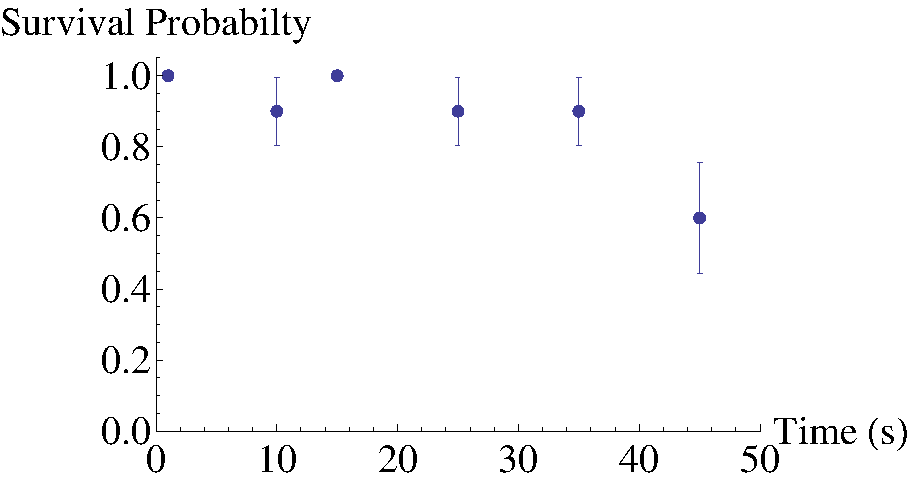
\includegraphics[width=0.45\textwidth]{lifetime-midarm1} \\
	Loading Hole &
	Along Y-Trap Rail \\
\end{tabular*}}
\end{frame}

\begin{frame}{Experimental Results - Secular Frequency}
Adding an additional frequency to the rf rails allows us to directly drive the 
secular motion of the ion to find its frequency.
\par\medskip
\centerline{\begin{tabular*}{0.9\textwidth}{cccc}
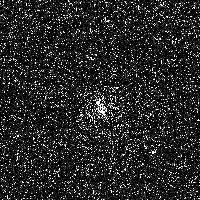
\includegraphics[width=0.1\textwidth]{axial/crop171} &
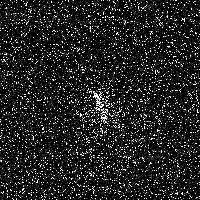
\includegraphics[width=0.1\textwidth]{axial/crop173} &
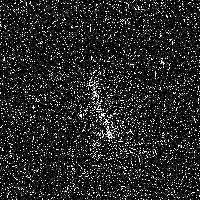
\includegraphics[width=0.1\textwidth]{axial/crop176} &
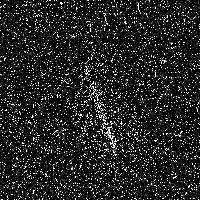
\includegraphics[width=0.1\textwidth]{axial/crop178} \\
{\small 24.171 MHz} & {\small 24.173 MHz} & {\small 24.176 MHz} & {\small 24.178 MHz} \\ 
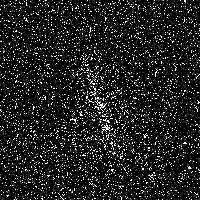
\includegraphics[width=0.1\textwidth]{axial/crop181} &
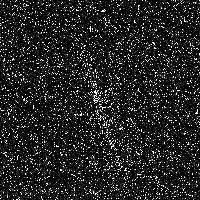
\includegraphics[width=0.1\textwidth]{axial/crop183} &
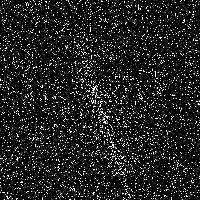
\includegraphics[width=0.1\textwidth]{axial/crop185} &
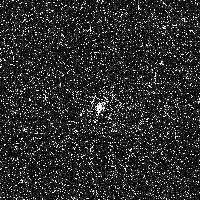
\includegraphics[width=0.1\textwidth]{axial/crop187} \\
{\small 24.181 MHz} & {\small 24.183 MHz} & {\small 24.185 MHz} & {\small 24.187 MHz} \\ 
\end{tabular*}}
\[w_{axial} \approx 0.75 MHz, w_{radial} \approx 1.50 MHz?, 2.05 MHz\]
\end{frame}

\begin{frame}{Experimental Results - Micromotion Compensation}
This secular frequency measurement is also sensitive to
our ion micromotion.
\begin{columns}
\begin{column}{0.4\textwidth}
	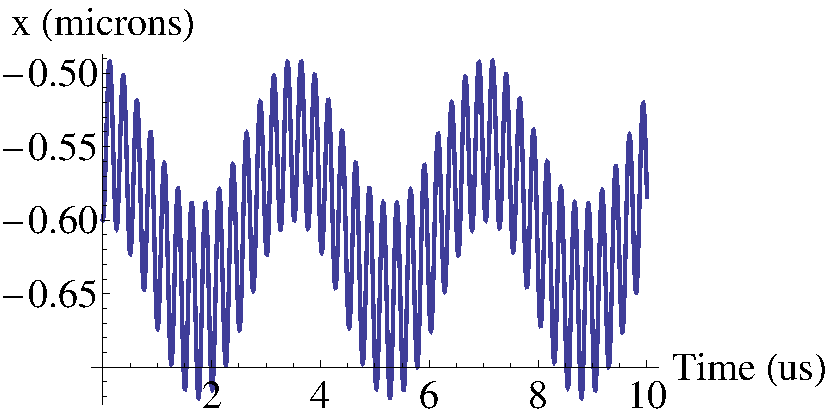
\includegraphics[height=0.35\textheight]{PaulTrap-micromotion}
\end{column}
\begin{column}{0.6\textwidth}
\begin{itemize}
	\item To the extent ion undergoes micromotion it sees the mixed
		signal between the trap rf and injected rf
	\item Provides a signal for fine tuning micromotion compensation
		in all 3 trap axes unlike most laser based schemes
	\item Measured stray fields in the loading hole of \(\approx 400V/m\)
\end{itemize}
\end{column}
\end{columns}
\end{frame}

\subsection{Mixed Species}
\begin{frame}{Experimental Results - Mixed Species}
Within the MUSIQC architecture we plan to have local motional gates between ions in the same trap and remote entanglement via photons to couple multiple traps.
\begin{itemize}
	\item Light from Barium's cooling transition (493nm) is easily transferred long distances via optical fiber
	\item Yb-171 has long lived hyperfine states that can easily be frequency initialized and used for motional gates
	\item By separating these tasks to different species the possibility for crosstalk is reduced
\end{itemize}
\end{frame}

\begin{frame}{Experimental Results - Mixed Species Progress}
\begin{columns}
	\begin{column}{0.4\textwidth}
		\centerline{\includegraphics[width=0.9\textwidth]%
			{BaYb}}
	\end{column}
	\begin{column}{0.6\textwidth}
		\begin{itemize}
			\item Crystal contains two cooled, bright Ba ions and one dark Yb ion
			\item Secular frequency shift has been measured to confirm the presence of Yb
			\item Yb ions are loaded via charge exchange with trapped Ba ions
			\item Need to further study cooling efficiency of long mixed species chains
		\end{itemize}
	\end{column}
\end{columns}
\end{frame}

\section[Future]{Future Directions}
\subsection{Mixed Species Normal Modes}
\begin{frame}{Future Directions - Cooling Ba+ and Yb+}
\begin{columns}
\begin{column}{0.4\textwidth}
	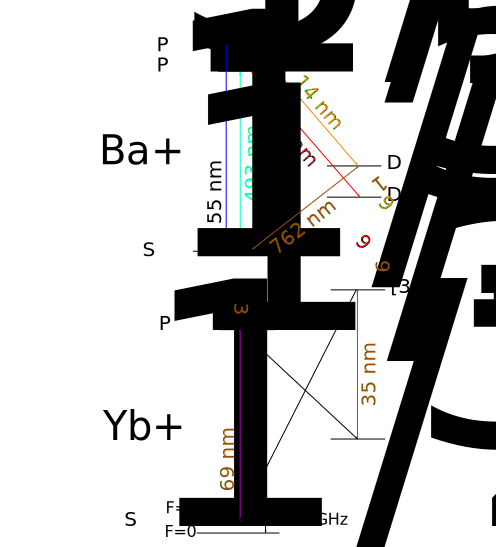
\includegraphics[height=0.7\textheight]{energylevels-BaYb}
\end{column}
\begin{column}{0.6\textwidth}
	\begin{itemize}
		\item Both species have accessible cooling cycles and dark states that can be used to readout quantum information
		\item Plan to build ECDLs at 369nm and 935nm
		\item Test chain reordering and mixed species chains in a surface trap
		\item Investigate continuous cooling of ion chain with Ba
	\end{itemize}
\end{column}
\end{columns}
\end{frame}

\begin{frame}{Future Directions - Mixed Species Normal Modes}
Trapping different mass ions in the same potential causes the normal
modes of the different species to decouple.
\par\medskip
\begin{tabular*}{1.0\textwidth}{@{\extracolsep{\fill}} lr}
	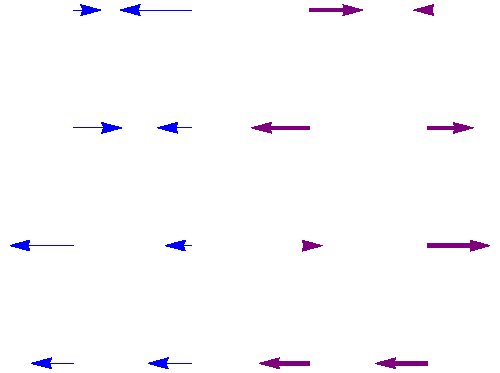
\includegraphics[width=0.4\textwidth]{Chains-BaYb_normal_modes} &
	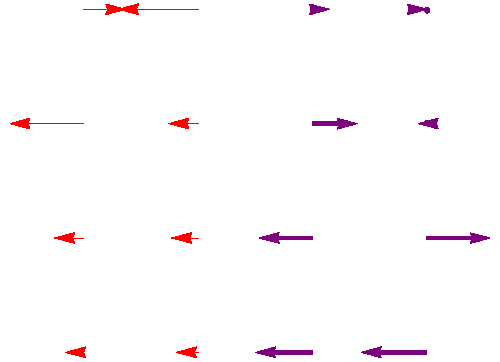
\includegraphics[width=0.4\textwidth]{Chains-CaYb_normal_modes} \\
	20\% mass difference (\textcolor{blue}{Ba}-\textcolor{mypurple}{Yb}) &
	300\% mass difference (\textcolor{red}{Ca}-\textcolor{mypurple}{Yb}) \\
\end{tabular*}
\end{frame}

\subsection{Raman Gates}
\begin{frame}{Future Directions - Coherent Manipulations}
\begin{columns}
	\begin{column}{0.4\textwidth}
		\centerline{\includegraphics[width=0.9\textwidth]%
			{Bloch_Sphere}}
	\end{column}
	\begin{column}{0.6\textwidth}
	\begin{itemize}
		\item Coherent rotations can easily be performed using coherent rf (Ba Zeeman levels) or microwave (Yb hyperfine levels) sources
		\item Corresponds to a rotation about the vector \( \hat{R} = \Omega \hat{x} + \delta \hat{z} \)
		\item Allows preparation of any separable state, but quantum computing is believed to require entanglement
	\end{itemize}
	\end{column}
\end{columns}
\end{frame}

\begin{frame}{Future Directions - Spin Motional Coupling}
\begin{columns}
	\begin{column}{0.3\textwidth}
	\begin{center}
		\includegraphics[height=0.4\textheight]{Raman-ciraczoller} \\
		{\small Required gate interactions}
	\end{center}
	\end{column}
	\begin{column}{0.7\textwidth}
		\begin{itemize}
			\item Cirac-Zoller 
				gate is an entangling controlled
				phase gate mediated by coupling to crystal motional modes
				\let\thefootnote\relax\footnote[frame]{J.I. Cirac and P. Zoller, PRL 74, 4091 (1995)}
			\item Requires cooling two ions to ground state of motional SHO
			\[(g_1\ket{\textcolor{blue}{g}}_1 + e_1\ket{\textcolor{red}{e}}_1) 
				(g_2\ket{\textcolor{blue}{g}}_2 + e_2\ket{\textcolor{red}{e}}_2)
				\ket{0} \]
			\item Allows quantum information transfer between Yb and Ba
		\end{itemize}
	\end{column}
\end{columns}
\end{frame}

\begin{frame}{Future Directions - Spin Motional Coupling}
Applying \(U_1 U_2 U_1\) implements the gate \\
\par\medskip
\begin{columns}
	\begin{column}{0.3\textwidth}
	\begin{center}
		\includegraphics[height=0.4\textheight]{Raman-ciraczoller} \\
	\end{center}
	\end{column}
	\begin{column}{0.7\textwidth}
	\begin{tabular}{ccc}
	\(\ket{g}_1\ket{g}_2\ket{0}\) & \(\;\) & \(\ket{g}_1\ket{g}_2\ket{0}\) \\
	\(\ket{g}_1\ket{e}_2\ket{0}\) & \(U_1\) & \(\ket{g}_1\ket{e}_2\ket{0}\) \\
	\(\ket{e}_1\ket{g}_2\ket{0}\) & \(\rightarrow\) & \(-i\ket{g}_1\ket{g}_2\ket{1}\) \\
	\(\ket{e}_1\ket{e}_2\ket{0}\) & \(\;\) & \(-i\ket{g}_1\ket{e}_2\ket{1}\) \\
	\end{tabular} \\
	\begin{tabular}{cccc}
	\(\;\) & \(\ket{g}_1\ket{g}_2\ket{0}\) & \(\;\) & \(\ket{g}_1\ket{g}_2\ket{0}\) \\
	\(U_2\) & \(\ket{g}_1\ket{e}_2\ket{0}\) & \(U_1\) & \(\ket{g}_1\ket{e}_2\ket{0}\) \\
	\(\rightarrow\) & \(i\ket{g}_1\ket{g}_2\ket{0}\) & \(\rightarrow\) & \(\ket{e}_1\ket{g}_2\ket{1}\) \\
	\(\;\) & \(-i\ket{g}_1\ket{e}_2\ket{0}\) & \(\;\) & \(-\ket{e}_1\ket{e}_2\ket{1}\) \\
	\end{tabular}
	\begin{itemize}
		\item Spin-motional coupling parametrized by \(\eta = k x\), small for rf and microwave photons
	\end{itemize}
	\end{column}
\end{columns}
\end{frame}

\begin{frame}{Future Directions - Raman Cirac-Zoller Gates}
\begin{columns}
	\begin{column}{0.5\textwidth}
		\centerline{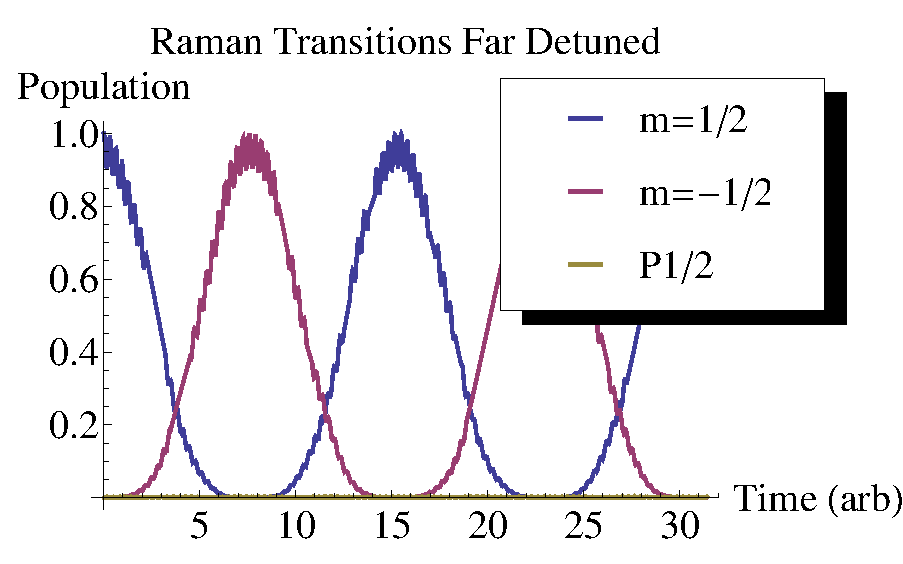
\includegraphics[height=0.4\textheight]{Raman-good}}
		\; \\
		\centerline{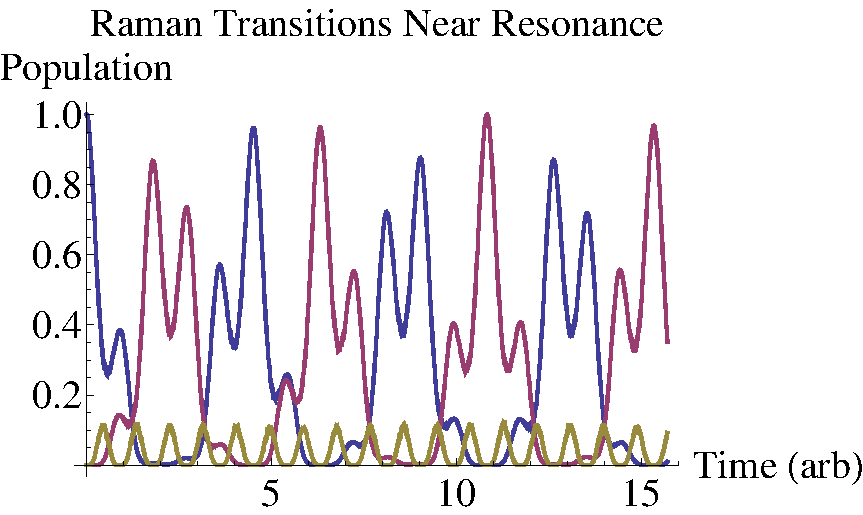
\includegraphics[height=0.38\textheight]{Raman-near_resonance}}
	\end{column}
	\begin{column}{0.5\textwidth}
		\centerline{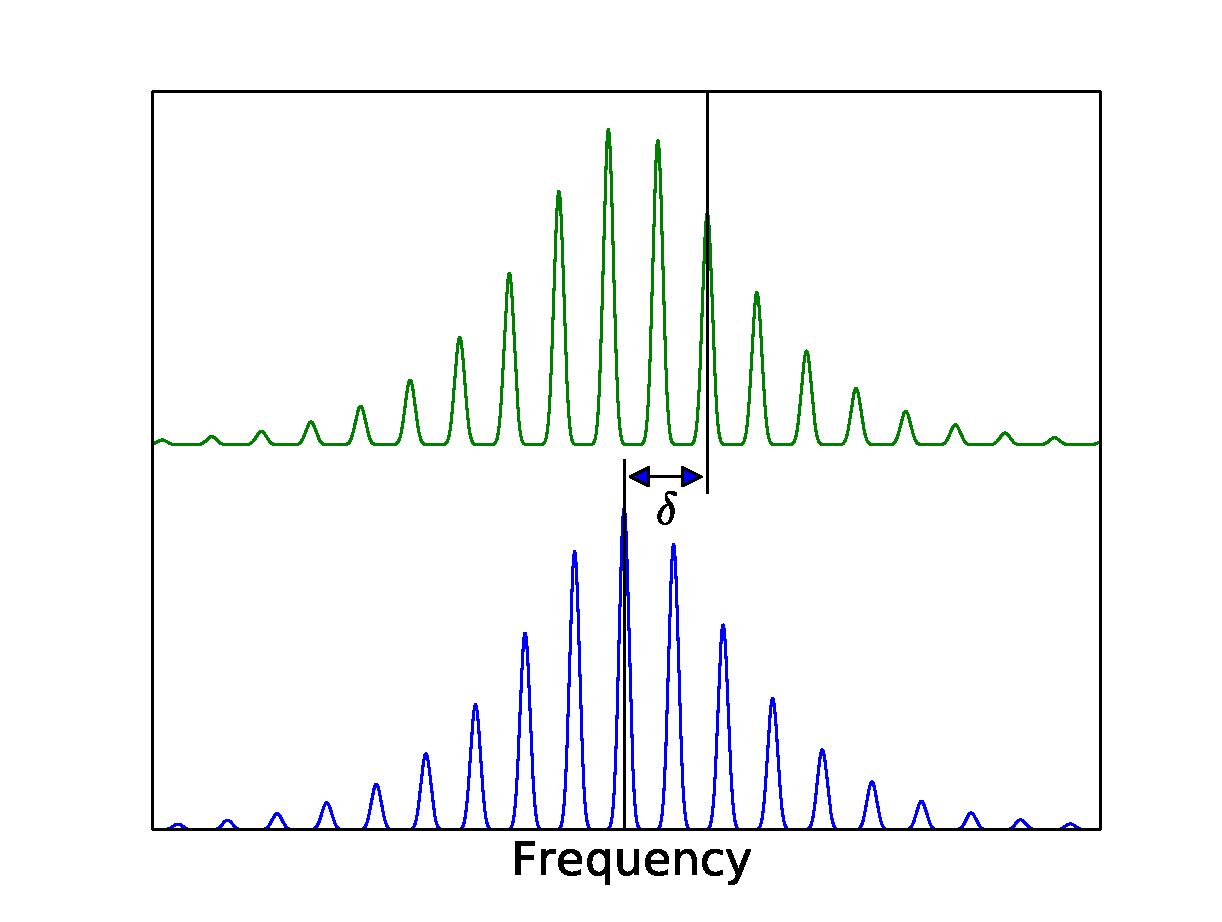
\includegraphics[height=0.55\textheight]{Raman}}
		\begin{eqnarray*}
			H_{1int} &=& \mu_1 E_1 \cos ( w t ) \\
			H_{2int} &=& \mu_2 E_2  \cos ( (w + w_{Z} ) t ) \\
			\Omega &=& \frac{\mu_1 E_1 \mu_2 E_2}{\Delta}
		\end{eqnarray*}
	\end{column}
\end{columns}
\end{frame}

\begin{frame}{Future Directions - Modelocked Millenia Laser}
\begin{columns}
	\begin{column}{0.4\textwidth}
		\centerline{\includegraphics[width=0.9\textwidth]%
			{Millennia}}
		\centerline{\includegraphics[width=0.9\textwidth]%
			{camera/millenia}}
	\end{column}
	\begin{column}{0.6\textwidth}
		\begin{itemize}
			\item Vanadate crystal pumped by 808~nm diode bars producing 2~W of 1064~nm modelocked light
			\item Semiconductor saturable absorber with picosecond
				relaxation times provides passive modelocking
			\item Large bandwidth allows transitions between hyperfine levels easily
		\end{itemize}
	\end{column}
\end{columns}
\end{frame}

\section[]{Conclusions}
\begin{frame}{Conclusions}
\begin{itemize}
	\item Quantum computing will allow for simulation of complicated
		physical systems and implementation of quantum algorithms
	\item Ions in surface traps present an implementation that can
		scale beyond 10s of qubits
	\item Raman motional gates and anharmonic surface traps are tools
		necessary to begin implementing these ideas, and we are approaching
		their realization
	\item Mixed ion species will provide a new technique to overcome some
		technical challenges and we are exploring its potential
\end{itemize}
\end{frame}

\begin{frame}{Thank You}
PI: Boris Blinov
\begin{block}{MUSQIC}
\begin{tabular*}{0.9\textwidth}{ccc}
Tomasz Sakrejda & Richard Graham & Zichao Zhou \\
\end{tabular*}
\end{block}

\begin{block}{Ion Trappers}
\begin{tabular*}{0.9\textwidth}{ccc}
Tom Noel & Carolyn Auchter & Chen-Kuan Chou \\
Matt Hoffman & Spencer Williams & Anupriya Jayakumar \\
Matt Bohman & Alexander Sivitilli
\end{tabular*}
\end{block}

\begin{columns}
\begin{column}{0.5\textwidth}
	
\includegraphics[width=0.9\textwidth]{musiqc_logo}
\end{column}
\begin{column}{0.5\textwidth}
	
\includegraphics[width=0.9\textwidth]{iarpa}
\end{column}
\end{columns}
\end{frame}

\end{document}
